\chapter{Desarrollo de la Solución}
Dentro de esta sección se expone con precisión el procedimiento descrito previamente en la sección anterior, correspondiente a cada acción incluida en la metodología implementada, junto con los entregables previstos.

\section{Adquisición de los Datos}

\textbf{Actividad 1 de “\textit{Adquisición de los Datos}”: Identificación de la data que contengan imágenes de rostros con características morfológicas faciales de proporciones similares}
 
Con el objetivo de entrenar un modelo de segmentación enfocado en características morfológicas faciales como arrugas y manchas, se llevó a cabo una exhaustiva búsqueda de bases de datos públicas en repositorios especializados. Se priorizó la recolección de conjuntos de datos que incluyeran imágenes faciales en alta resolución, variedad de edades, géneros y tonos de piel, así como condiciones de iluminación lo suficientemente controladas como para facilitar la segmentación de detalles faciales sutiles.

Durante este proceso, se identificaron diversos repositorios en plataformas como GitHub que ofrecían acceso a bases de datos con más de 200,000 imágenes faciales. Entre los conjuntos más destacados se encuentran versiones extendidas de datasets como CelebA, FFHQ (Flickr-Faces-HQ), y otros compendios curados por la comunidad investigadora, que contienen imágenes faciales etiquetadas o anotadas para tareas de reconocimiento y análisis facial.

Sin embargo, debido al enfoque específico de esta investigación la segmentación de características morfológicas finas como arrugas y manchas fue necesario realizar una selección cuidadosa de las imágenes más adecuadas. Para ello, se aplicaron criterios de claridad visual, resolución suficiente y visibilidad explícita de las deformaciones morfológicas faciales. Como resultado de este filtrado, se seleccionó un subconjunto compuesto por 20,000 imágenes faciales que cumplían con los siguientes criterios:

\begin{itemize}
    \item Alta calidad visual.   
    \item Visibilidad clara de texturas de la piel.
    \item Proporciones faciales dentro de un rango estándar para facilitar el modelado.
\end{itemize} 

Este conjunto reducido pero representativo, lo podemos ver en la Figura \ref{4:fig1}, constituye la base de entrenamiento y validación del modelo propuesto. La selección manual de estos datos buscó optimizar el desempeño del modelo, al exponerlo exclusivamente a ejemplos que contienen información útil para aprender patrones asociados a las características morfológicas de interés.

\begin{figure}[h]
	\begin{center}
		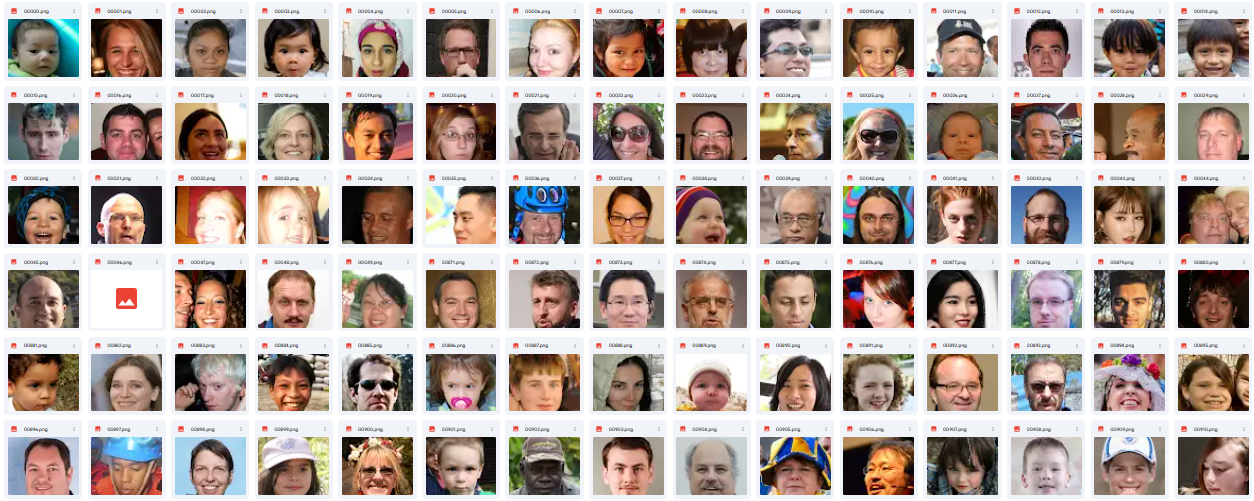
\includegraphics[width=0.75\textwidth]{4/figures/data.png}
		\caption[Dataset recolectado de repositorios]{Dataset recolectado de repositorios.\\
		Fuente: Elaboración propia}
		\label{4:fig1}
	\end{center}
\end{figure}

\section{Preprocesamiento de los Datos}

\textbf{Actividad 1 de “\textit{Preprocesamiento de los Datos}”: Filtración de imágenes faciales con características morfológicas}

Una vez recopilado el subconjunto de 20,000 imágenes faciales con características morfológicas visibles, se procedió a una etapa de filtración adicional orientada a reforzar la consistencia y la relevancia de los datos para la tarea de segmentación. Esta filtración se enfocó en garantizar que todas las imágenes seleccionadas contuvieran arrugas y manchas claramente identificables, descartando aquellas que, pese a su calidad visual, no presentaban estas características de manera explícita.

El proceso se realizó mediante una inspección semiautomática, apoyada en técnicas básicas de detección de texturas y realce de bordes para facilitar la identificación visual de las zonas con deformaciones. Como resultado, se aseguraron condiciones homogéneas entre las imágenes del dataset final de 5,000 imágenes, lo que permitió una base sólida para la generación de máscaras de segmentación precisas.

\textbf{Actividad 2 de “\textit{Preprocesamiento de los Datos}”: Representación y normalización de las imágenes faciales}

Con el conjunto de imágenes definitivo, se ejecutó un proceso de preprocesamiento estandarizado con dos objetivos principales: uniformar las dimensiones espaciales de las imágenes y generar las máscaras binarias asociadas a las regiones con deformaciones morfológicas.

En primer lugar, todas las imágenes fueron redimensionadas a una resolución uniforme de 1024x1024 píxeles, preservando la relación de aspecto y aplicando interpolación bilineal para mantener la calidad visual. Esta estandarización es fundamental para asegurar la compatibilidad estructural con las redes neuronales convolucionales utilizadas en etapas posteriores, y facilita la aplicación de operaciones convolucionales sobre áreas homogéneas.

En segundo lugar, se generaron máscaras binarias (en blanco y negro) correspondientes a cada imagen. Estas máscaras representan las regiones específicas del rostro que contienen arrugas, manchas u otras alteraciones morfológicas, codificadas de la siguiente manera:

\begin{itemize}
    \item Blanco (valor 1): Regiones con características morfológicas relevantes (objetivo de segmentación).   
    \item Negro (valor 0): Regiones sin interés morfológico.
\end{itemize} 

Las máscaras, como se ve en la Figura \ref{4:fig2}, fueron elaboradas a partir de una combinación de anotación semiautomática y herramientas de realce de texturas, contrastes y gradientes, con verificación manual en una muestra aleatoria para asegurar su validez.

\begin{figure}[h]
	\begin{center}
		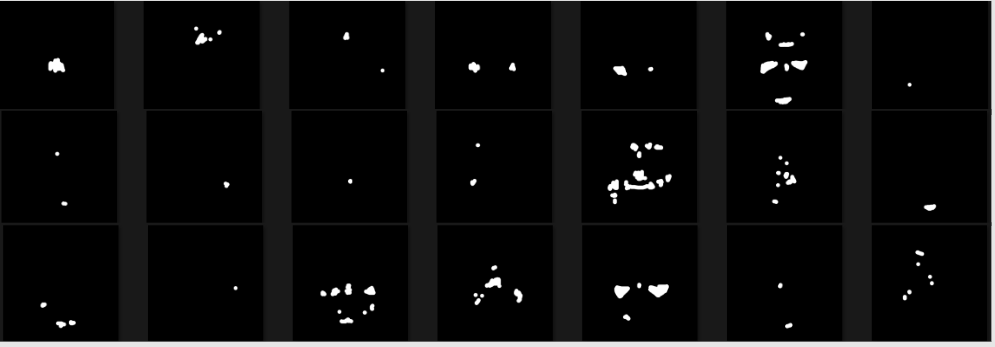
\includegraphics[width=0.75\textwidth]{4/figures/mascaras.png}
		\caption[Máscaras binarias generadas]{Máscaras binarias generadas.\\
		Fuente: Elaboración propia}
		\label{4:fig2}
	\end{center}
\end{figure}

Este proceso de representación y normalización, como se ve en el diagrama final de Preprocesamiento en la Figura \ref{4:fig3}, permitió convertir los datos originales en pares de entrada (imagen facial) y salida (máscara de segmentación), aptos para el entrenamiento supervisado del modelo de segmentación basado en redes neuronales convolucionales.

\begin{figure}[h]
	\begin{center}
		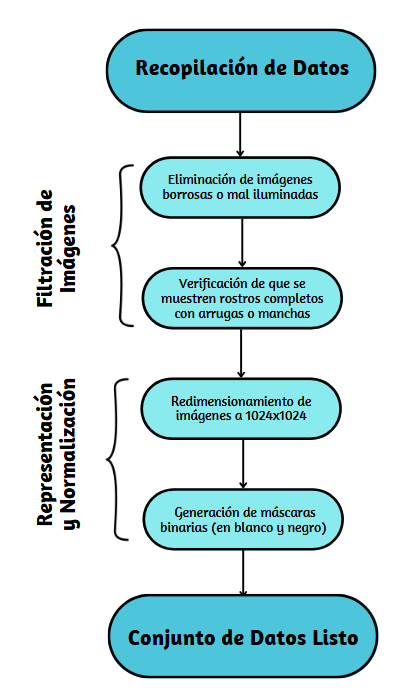
\includegraphics[width=0.75\textwidth]{4/figures/diagrama final prepo.png}
		\caption[Diagrama de Preprocesamiento Utilizado]{Diagrama de Preprocesamiento Utilizado.\\
		Fuente: Elaboración propia}
		\label{4:fig3}
	\end{center}
\end{figure}
\clearpage
\newpage
\section{Desarrollo de los Modelos de Segmentación}

\begin{enumerate}
  \item \textbf{Modelo de Segmentación: U-Net}
  \begin{figure}[H]
	\begin{center}
		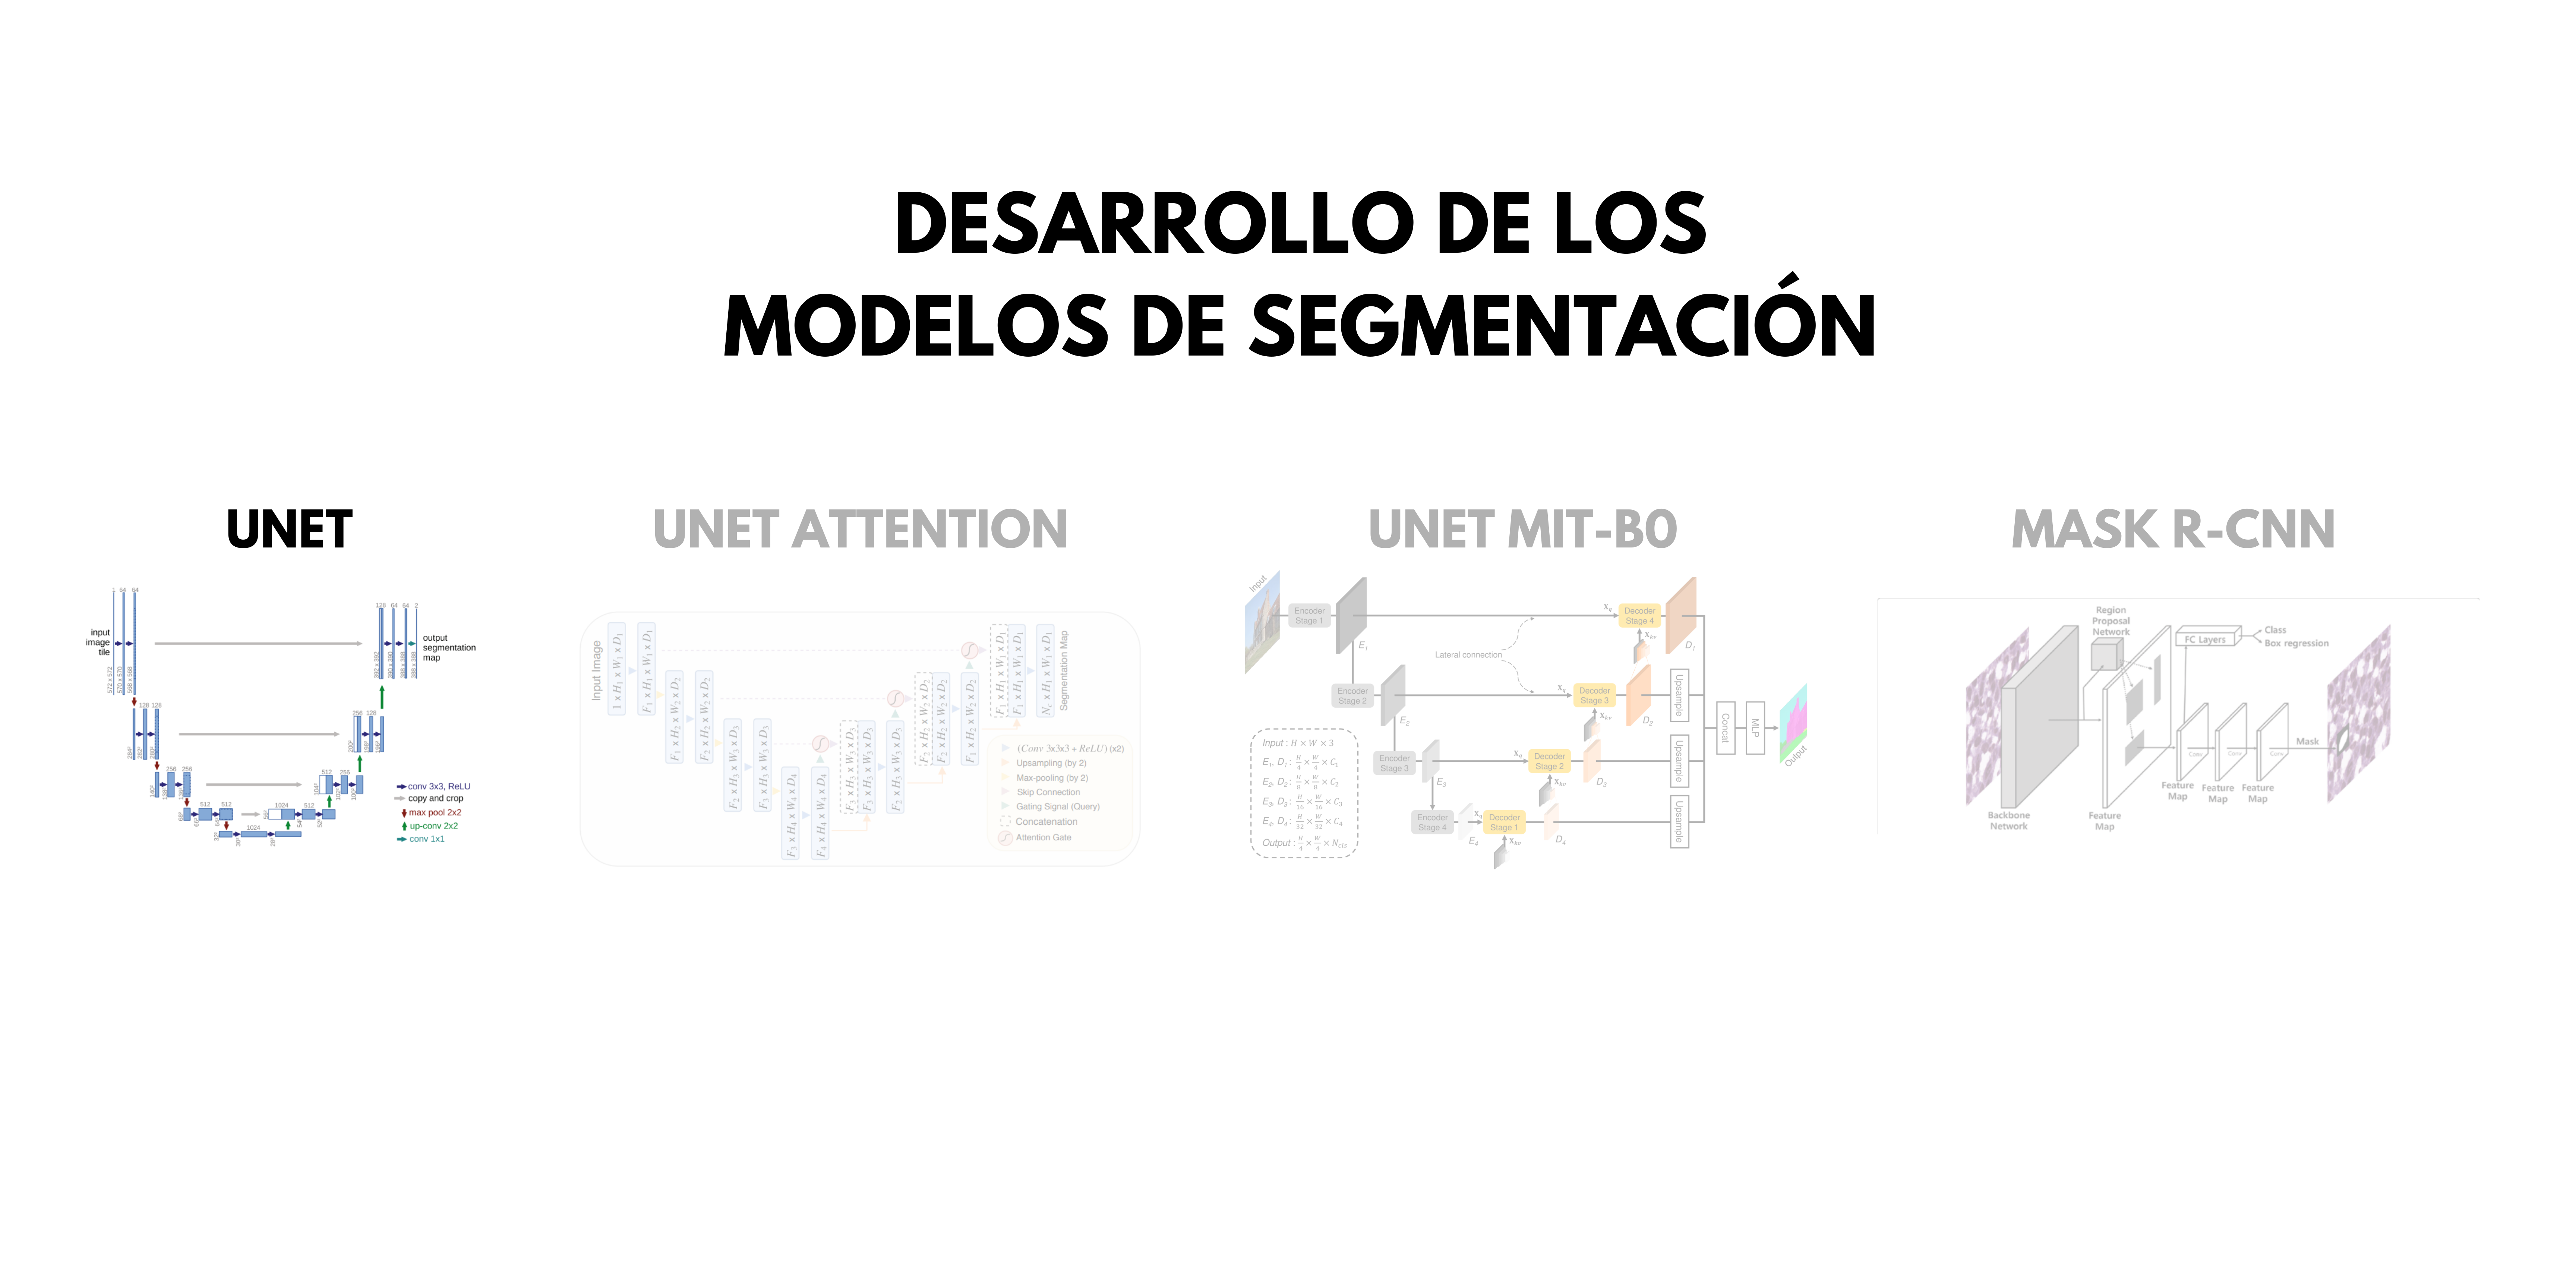
\includegraphics[width=1\textwidth]{4/figures/desunet.png}
		\caption[Desarrollo del Modelo U-Net]{Desarrollo del Modelo U-Net.\\
		Fuente: Elaboración propia}
		\label{4:figdesunet}
	\end{center}
\end{figure}
  \begin{itemize}

  \item\textbf{Actividad 1 de “\textit{Desarrollo de los Modelos de Segmentación}”: Diseño de la arquitectura del modelo}
\\
  Se implementó una arquitectura U-Net para segmentación de imágenes, con una estructura simétrica compuesta por un codificador (encoder) y un decodificador (decoder) unidos por conexiones de salto (skip connections).
\begin{itemize}
\item \textbf{Encoder:} Extrae características mediante bloques de convolución (dos capas con filtros 3x3, BatchNorm y ReLU) y reduce la resolución con max pooling. Produce mapas de características en escalas progresivamente más profundas: 64, 128, 256 y 512 canales.
\item \textbf{Bottleneck:} Máxima abstracción con 1024 mapas de características, sin max pooling para preservar la resolución.
\item \textbf{Decoder:} Reconstruye la imagen con convoluciones transpuestas para aumentar resolución, combinando información con el encoder mediante concatenaciones.
\item \textbf{Capa final:} Convolución $1\times1$ para generar la segmentación con 3 canales de salida.
\item \textbf{Pseudocódigo del Modelo:}

\begin{verbatim}
Input: Imagen X (3 canales)

e1 = enc1(X)  # Primer bloque de convolución
e2 = enc2(pool1(e1))  # Segundo bloque de convolución
e3 = enc3(pool2(e2))  # Tercer bloque de convolución
e4 = enc4(pool3(e3))  # Cuarto bloque de convolución

b = bottleneck(pool4(e4))  # Bottleneck, no max pooling

d4 = upconv4(b)  # Expansión con convolución transpuesta
d4 = dec4(concat(d4, e4))  # Conexión de salto con e4
d3 = upconv3(d4)  # Expansión con convolución transpuesta
d3 = dec3(concat(d3, e3))  # Conexión de salto con e3
d2 = upconv2(d3)  # Expansión con convolución transpuesta
d2 = dec2(concat(d2, e2))  # Conexión de salto con e2
d1 = upconv1(d2)  # Expansión con convolución transpuesta
d1 = dec1(concat(d1, e1))  # Conexión de salto con e1

Output = final_conv(d1)  # Capa final de convolución
\end{verbatim}

\end{itemize}



  \item\textbf{Actividad 2 “\textit{Desarrollo de los Modelos de Segmentación}”: Definición de componentes del modelo}
  \begin{itemize}
    \item \textbf{Clase Dataset personalizado:} Carga imágenes de rostros y máscaras binarias para arrugas y manchas, generando máscaras multiclase con valores {0: fondo, 1: arrugas, 2: manchas}. Se aplican transformaciones con Albumentations para robustecer el modelo (flip, rotación, brillo, cambio de tamaño, tensorización).
    \item \textbf{Modelo \texttt{U-Net}:} Detalla capas del encoder, bottleneck y decoder con su función en la reducción y recuperación de resolución y profundidad, con la capa final que produce un tensor de salida con 3 canales (una por clase).
    \item \textbf{Resumen de interacción entre componentes:} El dataset prepara las muestras; las imágenes se normalizan y las máscaras se convierten para usar cross-entropy. El modelo predice mapas segmentados, y la pérdida se calcula para actualizar pesos. La validación mide la capacidad de distinguir las clases en datos no vistos.
  \end{itemize}
\end{itemize}

  \newpage
  \item \textbf{Modelo de Segmentación: U-Net Attention}
  \begin{figure}[H]
	\begin{center}
		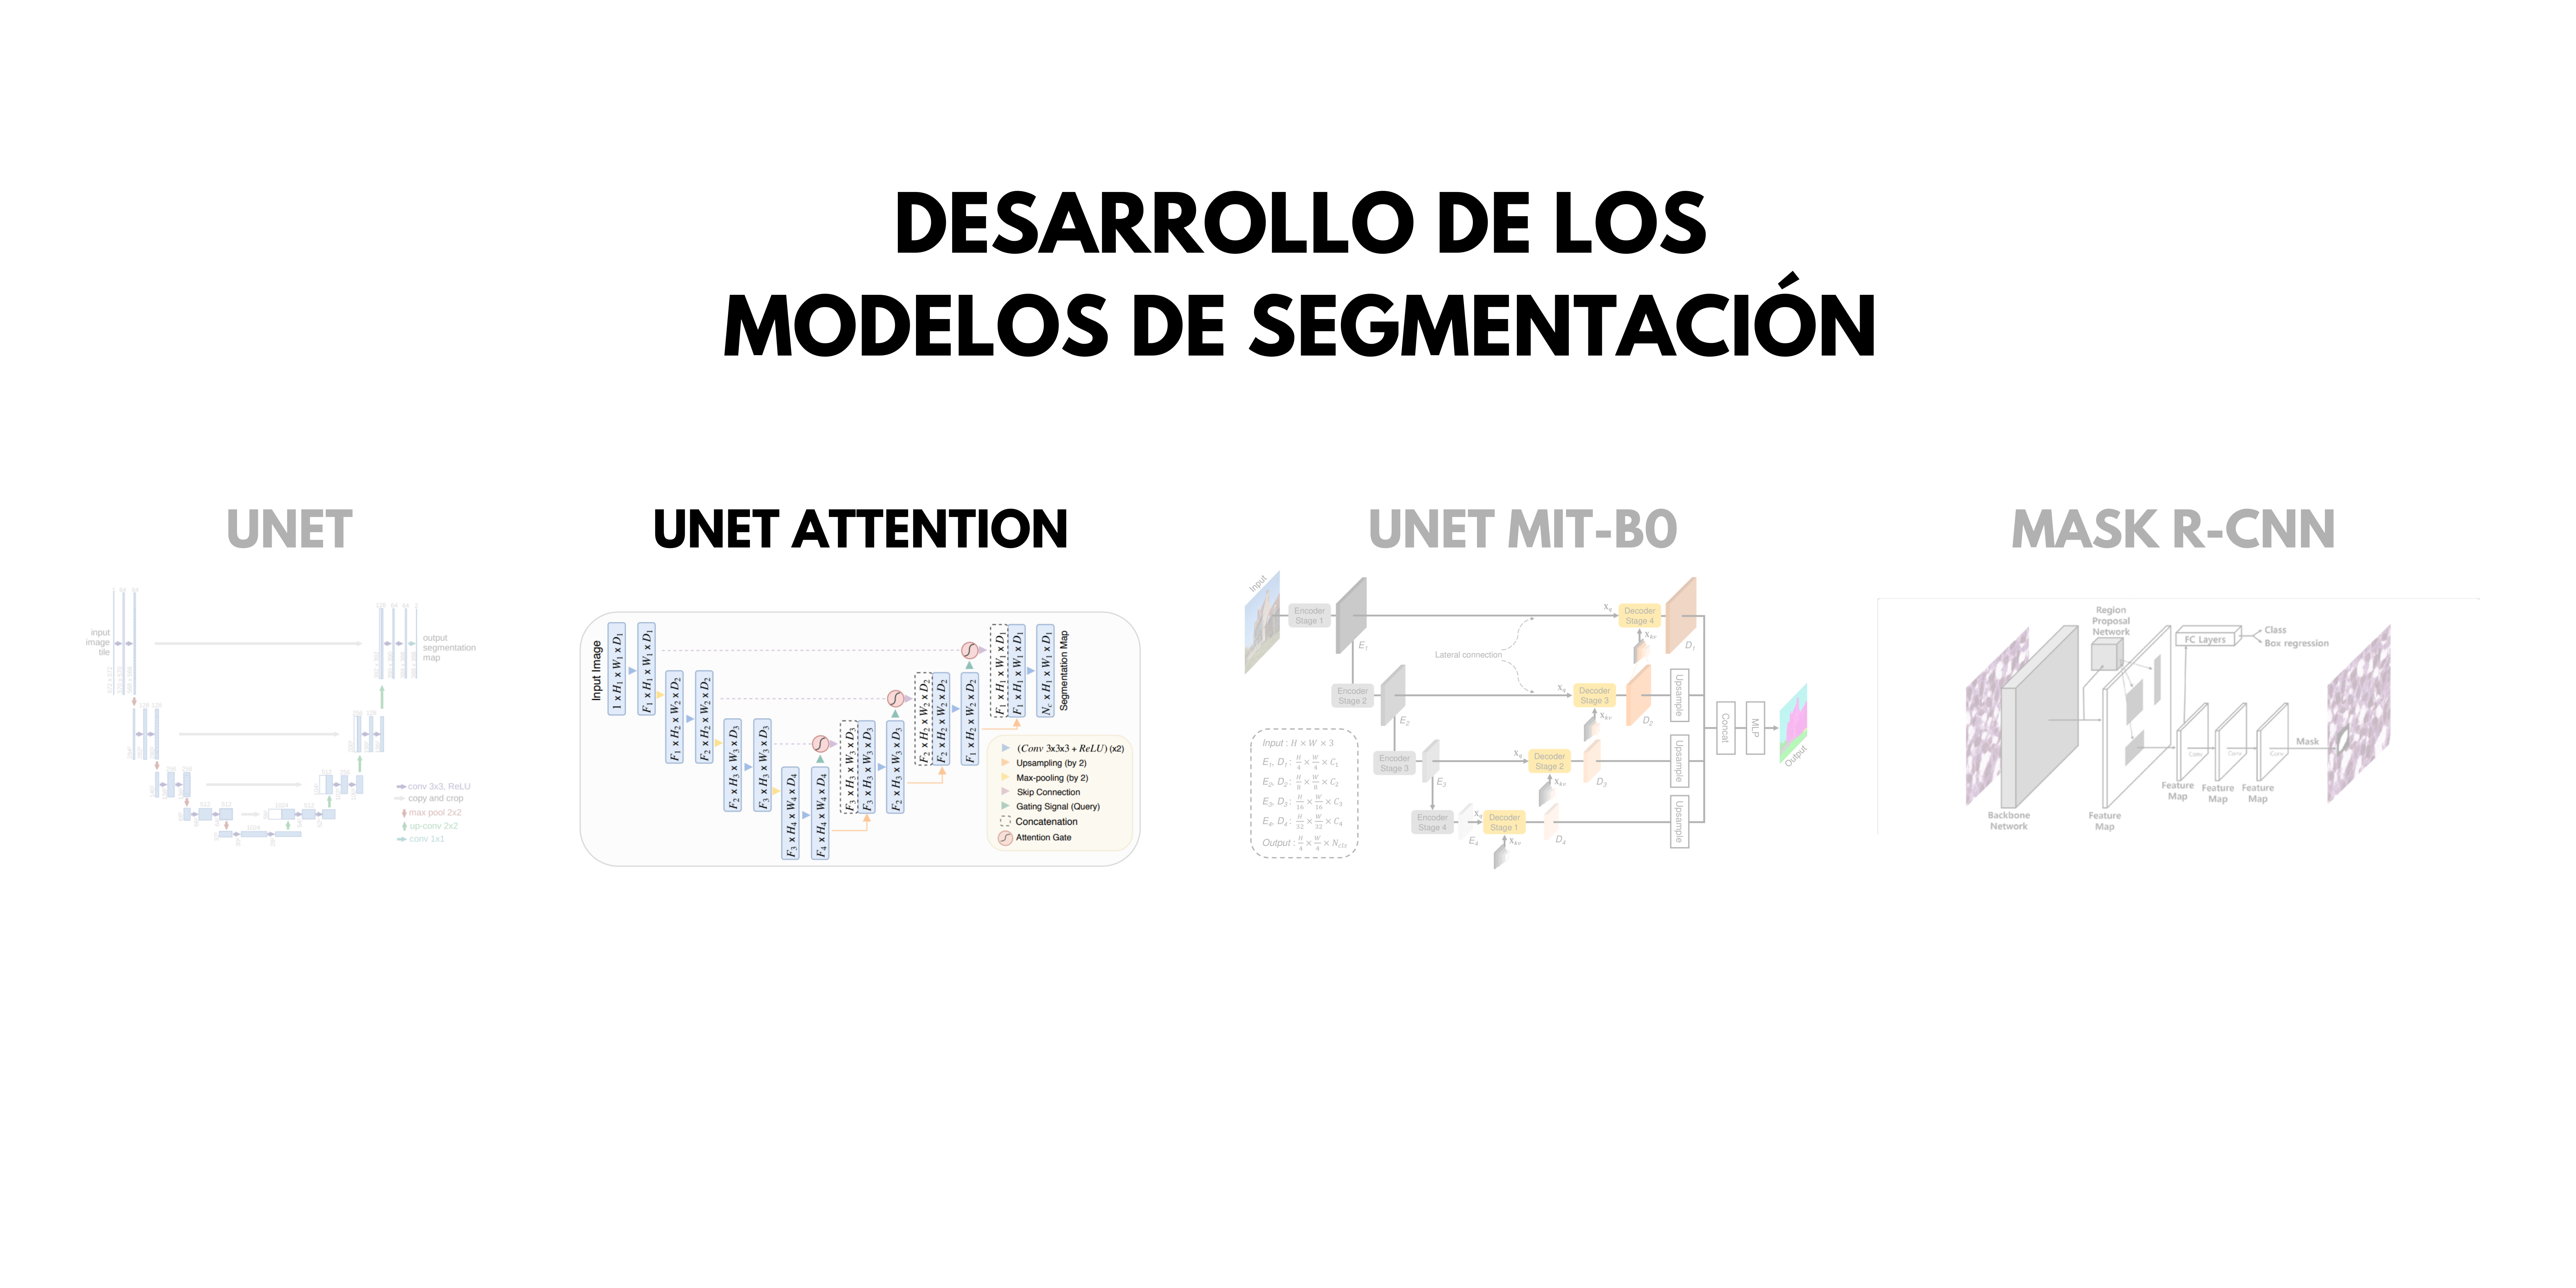
\includegraphics[width=1\textwidth]{4/figures/desunetat.png}
		\caption[Desarrollo del Modelo U-Net Attention]{Desarrollo del Modelo U-Net Attention.\\
		Fuente: Elaboración propia}
		\label{4:figdesunetat}
	\end{center}
\end{figure}
  \begin{itemize}


  \item\textbf{Actividad 1 de “\textit{Desarrollo de los Modelos de Segmentación}”: Diseño de la arquitectura del modelo}
\\
  Se propone un modelo U-Net con atención (\texttt{UNetAttention}), que combina un encoder-decoder simétrico con puertas de atención (\texttt{AttentionGate}) para resaltar regiones relevantes en la imagen.
\begin{itemize}
\item \textbf{Encoder:} Cuatro bloques \texttt{DoubleConv} (doble convolución + BatchNorm + ReLU), con reducción progresiva de resolución mediante \texttt{MaxPool2d(2)}. Los canales aumentan de 3 (RGB) a 64, 128, 256 y 512, capturando desde características básicas hasta patrones complejos y globales.
\item \textbf{Bottleneck:} Capa \texttt{DoubleConv} que expande de 512 a 1024 canales, condensando la información.
\item \textbf{Puertas de atención:} En lugar de conexiones directas, filtran la señal del encoder usando la información del decoder, mediante convoluciones 1×1, activaciones ReLU y sigmoid, generando un mapa de atención que multiplica la señal para conservar solo características relevantes.
\item \textbf{Decoder:} Upsampling con convoluciones transpuestas, concatenación con la salida del encoder filtrada por atención, y procesamiento con \texttt{DoubleConv}. Va de 1024 a 64 canales, reconstruyendo la segmentación paso a paso.
\item \textbf{Capa final:} Convolución $1\times1$ para generar la segmentación con 3 canales de salida.
\item \textbf{Pseudocódigo del Modelo:}



\begin{verbatim}
Input: Imagen X

# Encoder
enc1 = DoubleConv(X)
enc2 = DoubleConv(MaxPool(enc1))
enc3 = DoubleConv(MaxPool(enc2))
enc4 = DoubleConv(MaxPool(enc3))

# Bottleneck
bottleneck = DoubleConv(MaxPool(enc4))

# Decoder con atención
up4 = UpConv(bottleneck)
att3 = AttentionGate(up4, enc4)
up4_cat = Concatenate(up4, att3)
dec4 = DoubleConv(up4_cat)

up3 = UpConv(dec4)
att2 = AttentionGate(up3, enc3)
up3_cat = Concatenate(up3, att2)
dec3 = DoubleConv(up3_cat)

up2 = UpConv(dec3)
att1 = AttentionGate(up2, enc2)
up2_cat = Concatenate(up2, att1)
dec2 = DoubleConv(up2_cat)

up1 = UpConv(dec2)
up1_cat = Concatenate(up1, enc1)
dec1 = DoubleConv(up1_cat)

# Salida final
Output = Conv1x1(dec1)
Return Output
\end{verbatim}

\end{itemize}



  \item\textbf{Actividad 2 de “\textit{Desarrollo de los Modelos de Segmentación}”: Definición de componentes del modelo}

  \begin{itemize}
    \item \textbf{DoubleConv:} Dos convoluciones seguidas de BatchNorm y ReLU para extracción eficiente y estable.
    \item \textbf{AttentionGate:} Módulo que recibe señales del encoder y decoder, reduce dimensionalidad, aplica activaciones y genera un mapa de atención que filtra características relevantes para mejorar precisión espacial.
    \item \textbf{UpConv (Transposed Convolution):} Upsampling aprendido para reconstruir resolución de manera precisa.
    \item \textbf{Conv1x1 final:} Reduce canales a 1 para salida binaria.
  \end{itemize}
  \end{itemize}
  \newpage
  \item \textbf{Modelo de Segmentación: U-Net con codificador MiT-B0 (Mix Transformer)}
  \begin{figure}[H]
	\begin{center}
		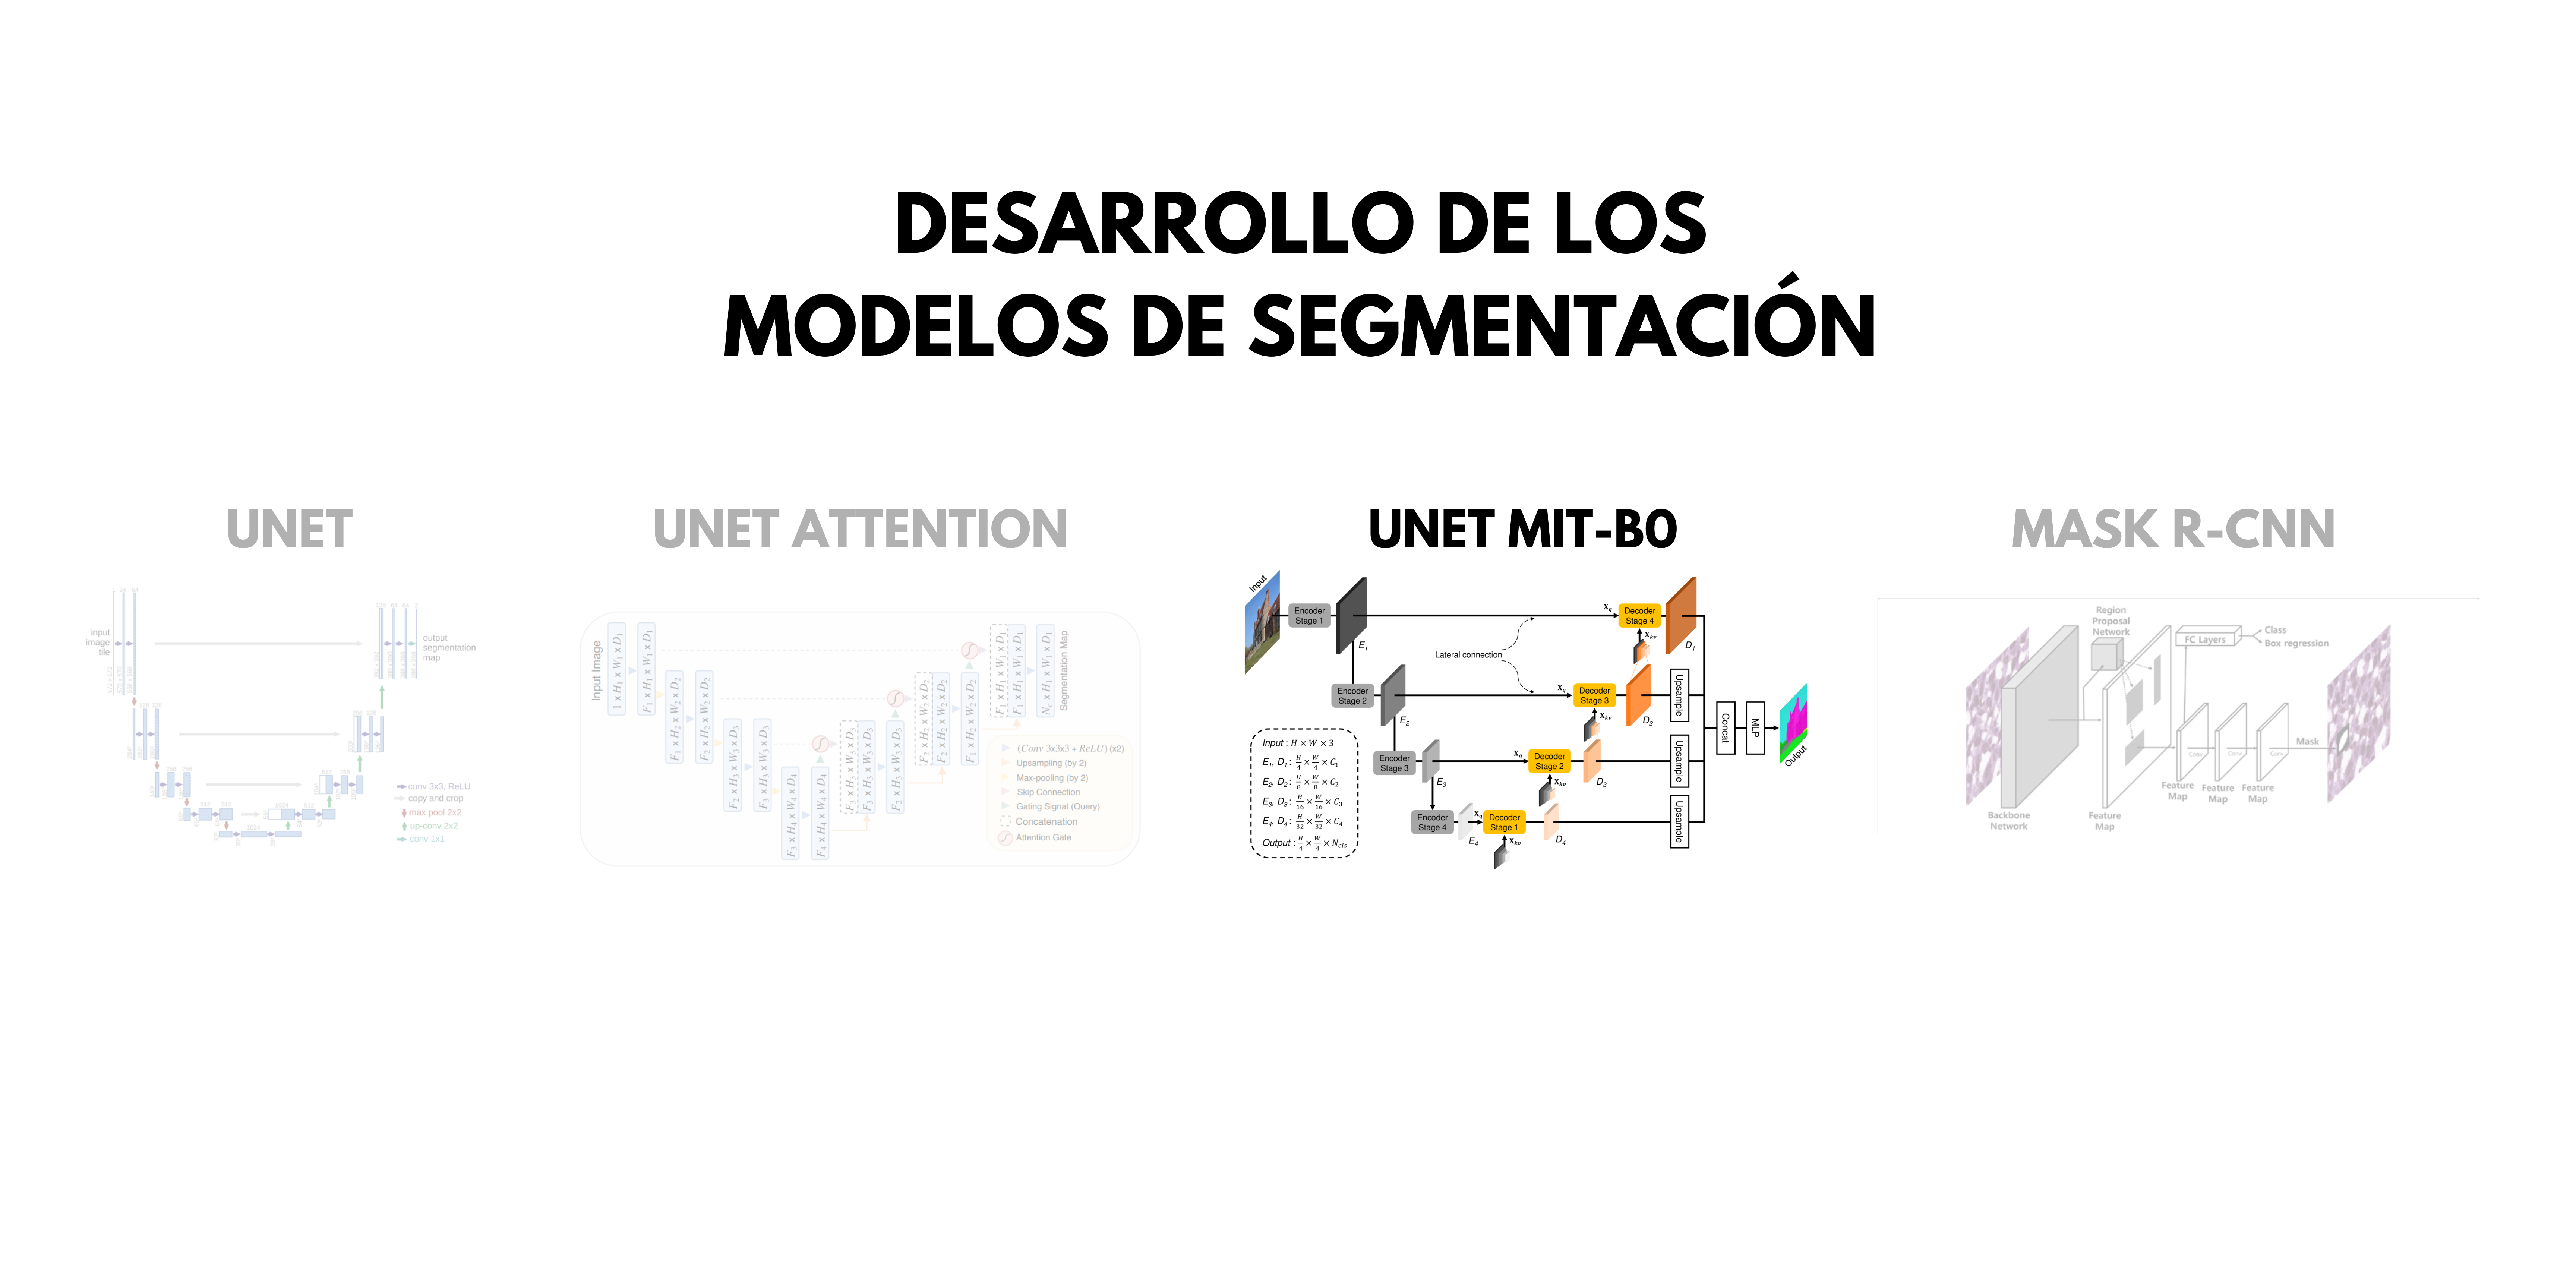
\includegraphics[width=1\textwidth]{4/figures/desunetmit.png}
		\caption[Desarrollo del Modelo U-Net con codificador MiT-B0]{Desarrollo del Modelo U-Net con codificador MiT-B0.\\
		Fuente: Elaboración propia}
		\label{4:figdesunetmit}
	\end{center}
\end{figure}
  \begin{itemize}

  \item\textbf{Actividad 1 de “\textit{Desarrollo de los Modelos de Segmentación}”: Diseño de la arquitectura del modelo}
\\
  El modelo \texttt{MiT-B0} (Mix Transformer) es una arquitectura de red neuronal que combina la estructura de U-Net con bloques de atención de tipo Transformer. Esta combinación permite al modelo capturar tanto características locales como globales en las imágenes, mejorando la segmentación en comparación con arquitecturas convencionales.

\begin{itemize}
\item \textbf{Encoder:} Consta de cuatro etapas jerárquicas que reducen progresivamente la resolución espacial mientras aumentan la profundidad de los mapas de características. Cada etapa emplea bloques Transformer con auto-atención eficiente. Las salidas se almacenan para conexiones de salto.
\item \textbf{Bottleneck:} Representa el mapa de características más profundo y abstracto del encoder. No contiene operaciones adicionales, pero actúa como cuello de botella de la arquitectura.
\item \textbf{Decoder:} Reconstruye la resolución original a través de cuatro etapas de upsampling. En cada etapa, se concatena la salida del encoder correspondiente mediante skip connections, combinando detalles espaciales y contexto.
\item \textbf{Capa final:} Convolución $1\times1$ transforma la salida del decoder en un tensor de logits por clase. Luego, se aplica \texttt{softmax} por píxel y se obtiene la predicción de clase con \texttt{argmax}.
\item \textbf{Pseudocódigo del Modelo:}

\begin{verbatim}
Input: Imagen X
# Encoder
enc1 = MiTBlock(X)
enc2 = MiTBlock(enc1)
enc3 = MiTBlock(enc2)
enc4 = MiTBlock(enc3)
# Bottleneck
bottleneck = MiTBlock(enc4)
# Decoder
up4 = UpConv(bottleneck)
att3 = AttentionGate(up4, enc4)
up4_cat = Concatenate(up4, att3)
dec4 = MiTBlock(up4_cat)
up3 = UpConv(dec4)
att2 = AttentionGate(up3, enc3)
up3_cat = Concatenate(up3, att2)
dec3 = MiTBlock(up3_cat)
up2 = UpConv(dec3)
att1 = AttentionGate(up2, enc2)
up2_cat = Concatenate(up2, att1)
dec2 = MiTBlock(up2_cat)
up1 = UpConv(dec2)
up1_cat = Concatenate(up1, enc1)
dec1 = MiTBlock(up1_cat)
# Salida final
Output = Conv1x1(dec1)
Return Output
\end{verbatim}
\end{itemize}
  \item\textbf{Actividad 2 de “\textit{Desarrollo de los Modelos de Segmentación}”: Definición de componentes del modelo}
  
  
  \begin{itemize}
    \item \textbf{FaceSegDataset:} Hereda de \texttt{torch.utils.data.Dataset}. Carga imágenes RGB, construye máscaras multiclase a partir de dos binarias (fondo=0, arrugas=1, manchas=2), aplica transformaciones de Albumentations (resize, rotación, brillo, normalización y conversión a tensor), y verifica la distribución de clases.
    \item \textbf{EarlyStopping:} Detiene el entrenamiento si la pérdida de validación no mejora tras 5 épocas (con \texttt{min\_delta=0}).
    \item \textbf{Transforms:} Pipelines separados para entrenamiento y validación, usando Albumentations.
    \item \textbf{collate\_fn:} Agrupa pares \texttt{(imagen, máscara)} en lotes mediante \texttt{torch.stack}.
    \item \textbf{compute\_metrics:} Calcula precisión (media y por clase), Dice Coefficient, e IoU.
    \item \textbf{Modelo (smp.Unet):} Instancia de \texttt{smp.Unet} con \texttt{encoder\_name='mit\_b0'}, pesos \texttt{imagenet}, y configuración para entrada RGB y 3 clases de salida.
\end{itemize}

  \end{itemize}

  \newpage
  \item \textbf{Modelo de Segmentación: Mask R-CNN}
  \begin{figure}[H]
	\begin{center}
		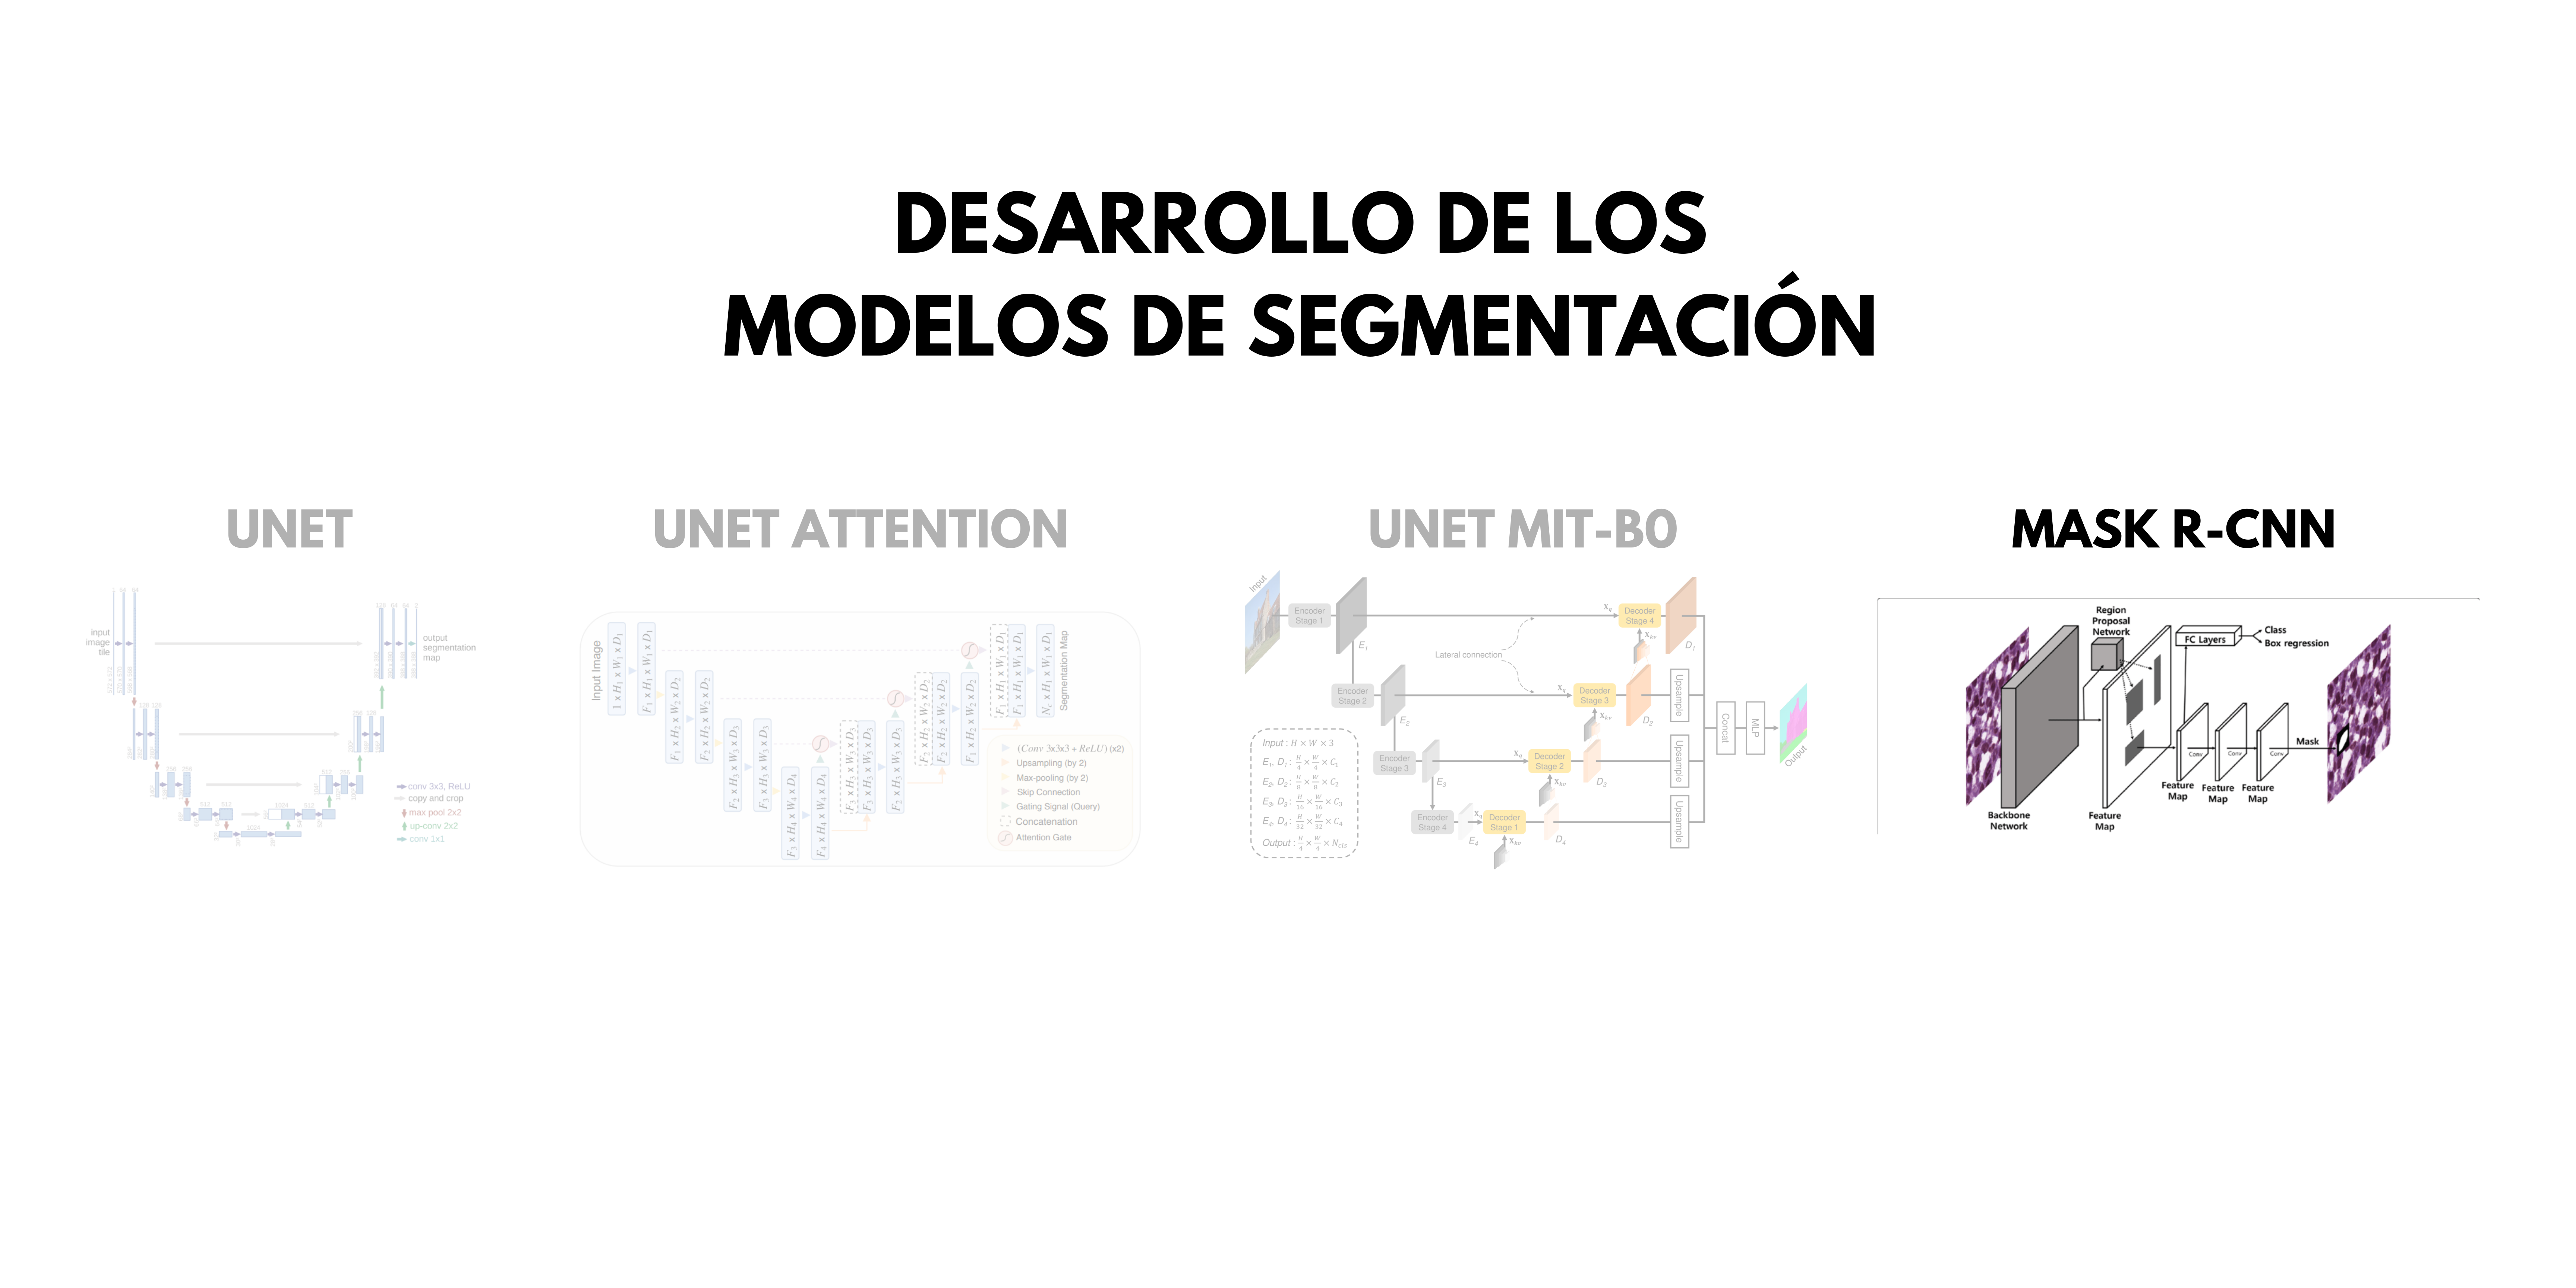
\includegraphics[width=1\textwidth]{4/figures/desmask.png}
		\caption[Desarrollo del Modelo Mask R-CNN]{Desarrollo del Modelo Mask R-CNN.\\
		Fuente: Elaboración propia}
		\label{4:figdesmask}
	\end{center}
\end{figure}
  \begin{itemize}

 
  \item\textbf{Actividad 1 de “\textit{Desarrollo de los Modelos de Segmentación}”: Diseño de la arquitectura del modelo}
\\
La arquitectura seleccionada para abordar la tarea de detección y segmentación de arrugas y manchas en imágenes faciales es la avanzada \textbf{Mask R-CNN}, reconocida por su capacidad para combinar detección de objetos (identificación y localización con cajas delimitadoras) y segmentación de instancias (precisión a nivel de píxel en cada objeto detectado). El diseño de la arquitectura considera los siguientes bloques fundamentales, organizados de forma jerárquica para maximizar la precisión multiescala y optimizar la eficiencia computacional:

\begin{itemize}
\item \textbf{Backbone:} ResNet-50 con FPN, que extrae características a múltiples escalas, combinando detalles espaciales y semánticos.

\item \textbf{Region Proposal Network (RPN):} Genera regiones candidatas (RoIs) a partir de mapas multiescala, utilizando anclas de distintos tamaños y formas.

\item \textbf{ROI Align:} Extrae regiones sin distorsión.

\item \textbf{Box Head:} Clasifica y ajusta cajas.

\item \textbf{Mask Head:} Genera máscaras binarias de $28 \times 28$ píxeles por clase.

\item \textbf{Pseudocódigo del Modelo:}

\begin{verbatim}
  Input: Imagen I
  
  # Backbone (ResNet-50 + FPN)
  F = FeaturePyramid(ResNet50(I))  
  
  # Region Proposal Network (RPN)
  anchors = GenerateAnchors(F)         
  proposals = []
  for anchor in anchors:
      obj_score, bbox_delta = RPNHead(anchor)  
      proposals.append(RefineAnchor(anchor, bbox_delta, obj_score))
  
  # Seleccionar N RoIs
  RoIs = SelectTopNProposals(proposals, N)
  
  # ROI Align
  aligned_features = []
  for roi in RoIs:
      aligned = ROIAlign(F, roi)
      aligned_features.append(aligned)
  
  # ROI Heads (Fast R-CNN Predictor)
  final_detections = []
  for feat in aligned_features:
      class_logits = ClassHead(feat)
      bbox = BBoxHead(feat)
      final_detections.append((class_logits, bbox))
  
  # Mask Head (Mask R-CNN Predictor)
  final_masks = []
  for i, (class_logits, bbox) in enumerate(final_detections):
      if IsObject(class_logits):  # No es clase fondo
          roi = RoIs[i]
          mask_feat = aligned_features[i]
          mask = MaskHead(mask_feat)
          resized_mask = ResizeMask(mask, bbox)
          final_masks.append((class_logits, bbox, resized_mask))
  
  # Salida final
  Output = final_masks
  Return Output
  \end{verbatim}
  
\end{itemize}

\item\textbf{Actividad 2 de “\textit{Desarrollo de los Modelos de Segmentación}”: Definición de componentes del modelo}
  

\begin{itemize}
    \item \textbf{Backbone:} ResNet-50 preentrenado en ImageNet, manteniendo las capas convolucionales y los bloques residuales. 
    
    \item \textbf{FPN:} Red lateral que toma las salidas de las etapas intermedias de ResNet-50 (conv2, conv3, conv4, conv5) para generar un conjunto de mapas de características enriquecidos a diferentes escalas.
    
    \item \textbf{RPN:} Subred de dos capas (una convolucional y dos salidas: clasificación de objeto/no objeto y regresión de anclas) que genera alrededor de 2000 propuestas por imagen.
    
    \item \textbf{ROI Align Layer:} Opera sobre las propuestas generadas para extraer regiones de interés correctamente alineadas, evitando distorsiones.
    
    \item \textbf{Box Predictor:} Dos capas densas (\textit{fully connected layers}) que predicen la clase de cada ROI y ajustan las coordenadas de las cajas delimitadoras.
    
    \item \textbf{Mask Predictor:} Tres capas convolucionales adicionales que generan máscaras de segmentación por clase, a partir de las características ROI alineadas.
    
    \item \textbf{Optimizador:} Adam con tasa de aprendizaje inicial $1 \times 10^{-4}$, seleccionado por su capacidad para manejar ajustes finos con datos ruidosos.
    
    \item \textbf{Funciones de pérdida:} La pérdida total combina tres componentes: 
    \begin{itemize}
        \item \textit{Classification Loss} (cross-entropy).
        \item \textit{Box Regression Loss} (smooth L1).
        \item \textit{Mask Loss} (binary cross-entropy a nivel de píxel).
    \end{itemize}
\end{itemize}

  \end{itemize}
\end{enumerate}


El proceso de Desarrollo de los Modelos de Segmentación que se siguió, se puede ver en el diagrama final de Desarrollo en la Figura \ref{4:figdesfin}.
\begin{figure}[h]
	\begin{center}
		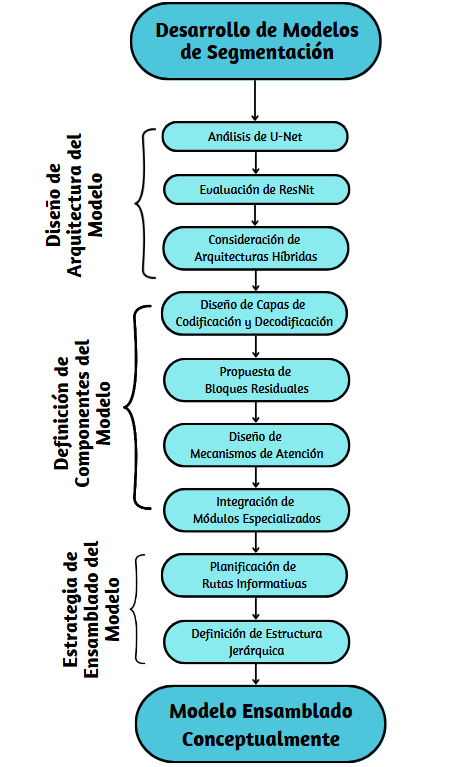
\includegraphics[width=0.75\textwidth]{4/figures/Diagrama de Desarrollo.png}
		\caption[Diagrama de Desarrollo Utilizado]{Diagrama de Desarrollo Utilizado.\\
		Fuente: Elaboración propia}
		\label{4:figdesfin}
	\end{center}
\end{figure}
\clearpage
\newpage

\section{Entrenamiento del modelo}

\begin{enumerate}
  \item \textbf{Modelo de Segmentación: U-Net}
  \begin{figure}[H]
	\begin{center}
		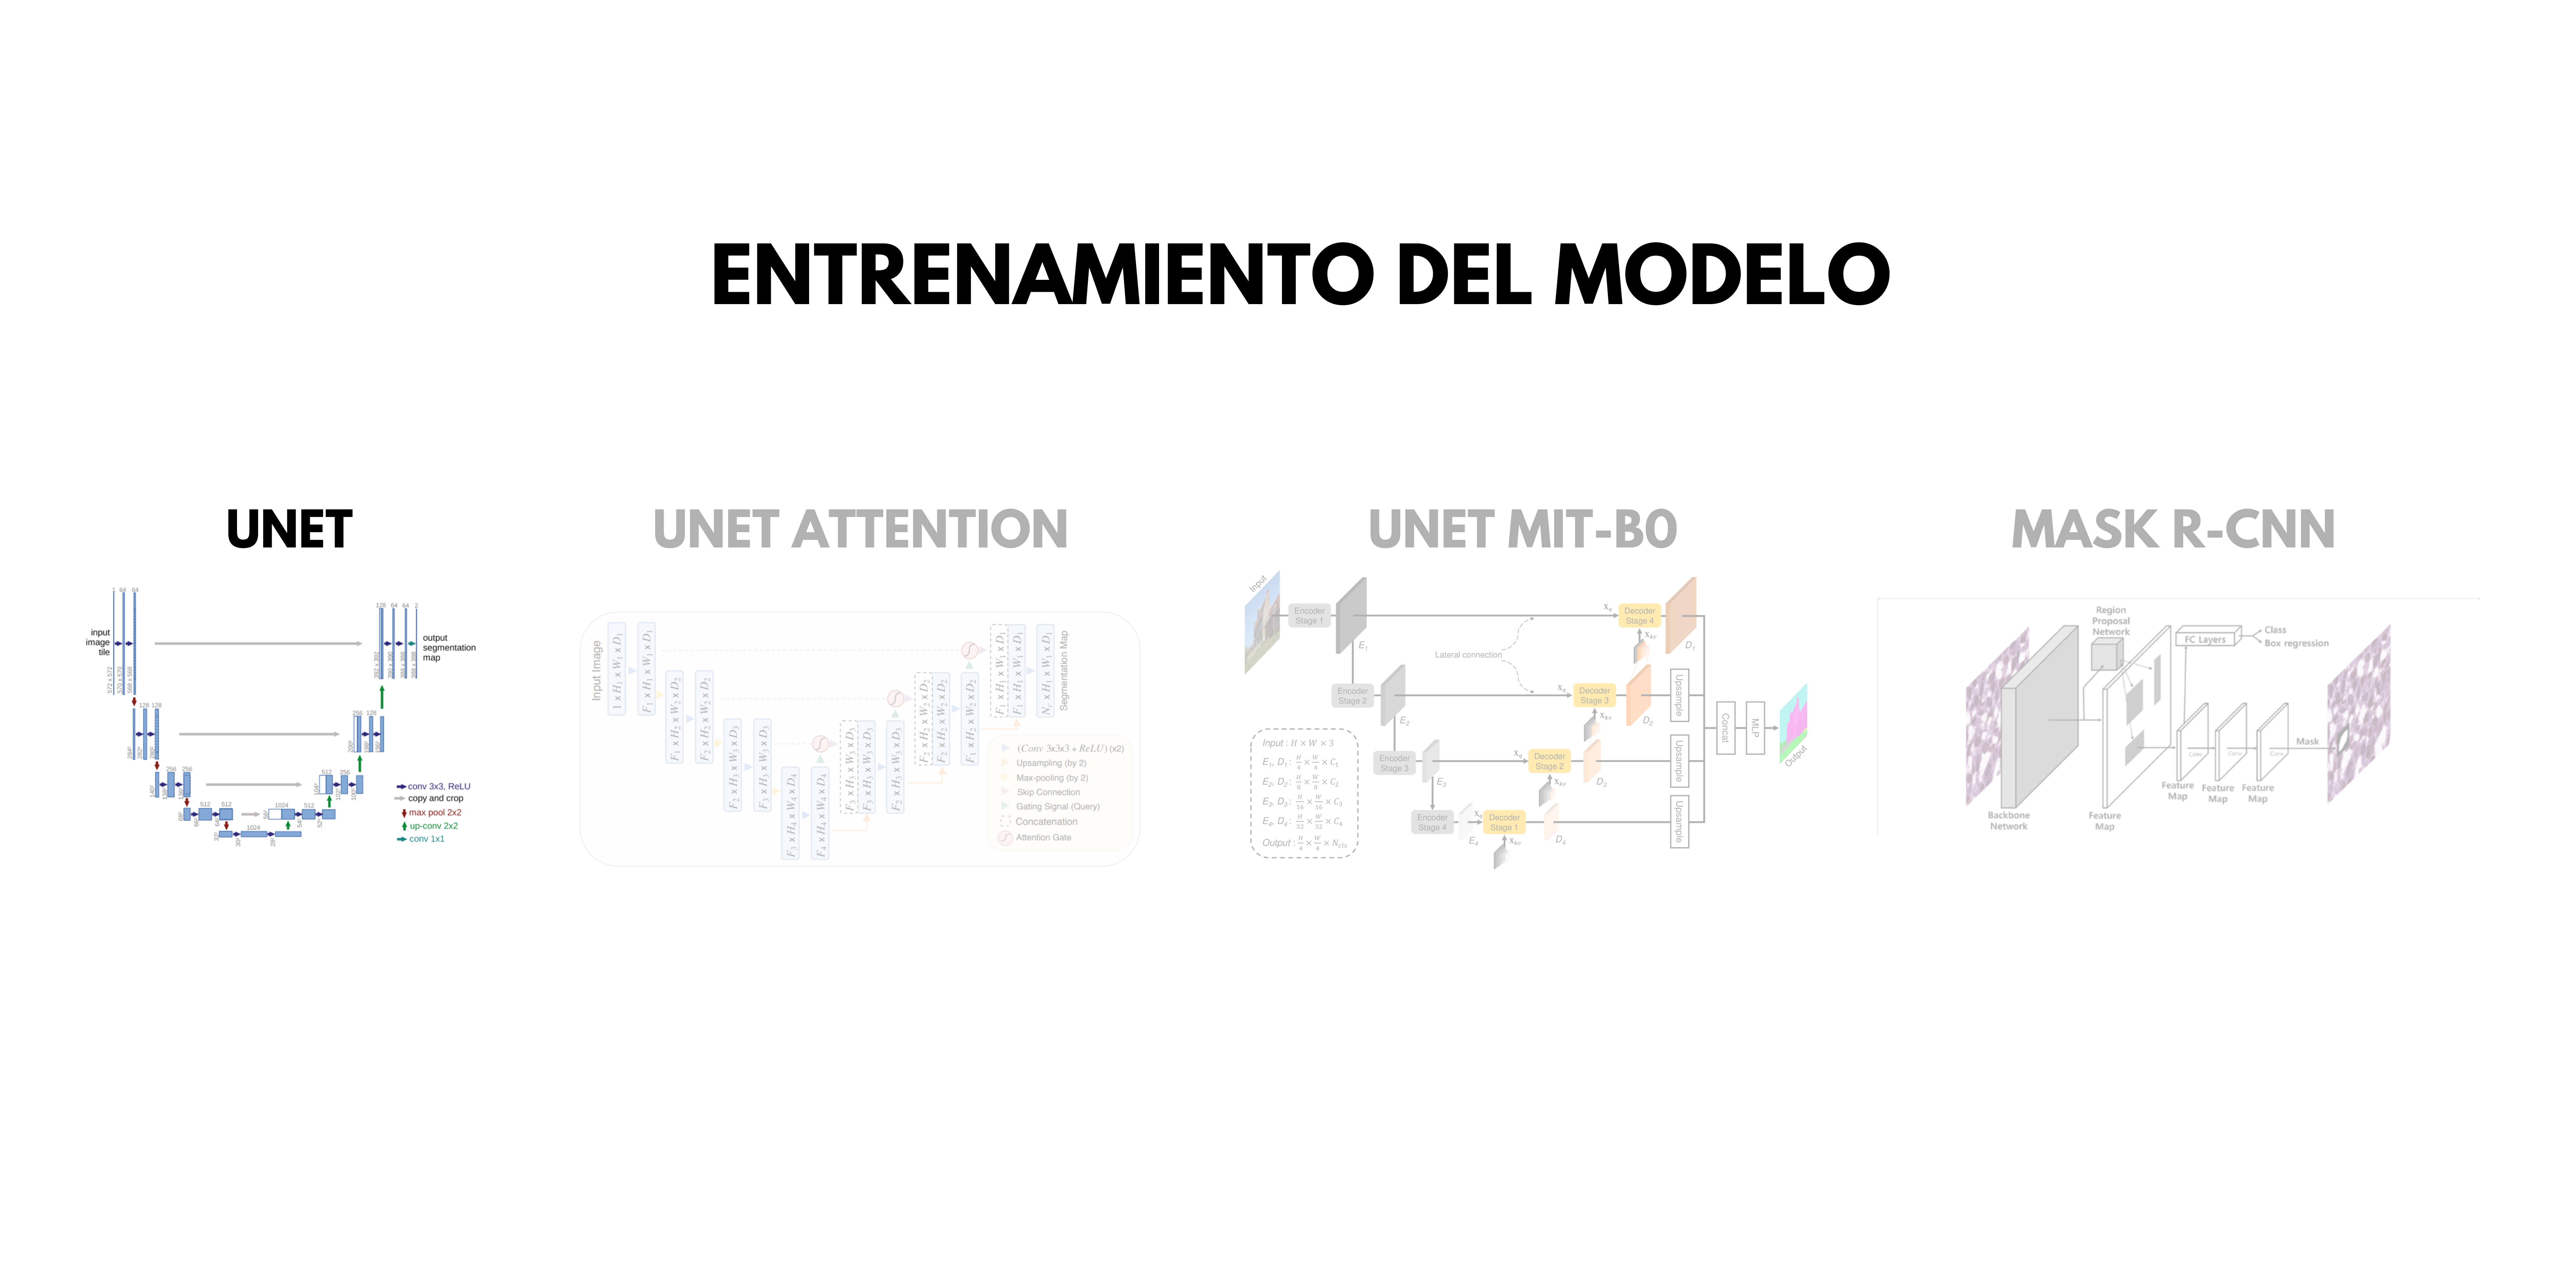
\includegraphics[width=1\textwidth]{4/figures/entrunet.png}
		\caption[Entrenamiento del Modelo U-Net]{Entrenamiento del Modelo U-Net.\\
		Fuente: Elaboración propia}
		\label{4:figentunet}
	\end{center}
\end{figure}
  \begin{itemize}
  \item\textbf{Actividad 1 de “\textit{Entrenamiento del modelo}”: Configuración del entorno de entrenamiento}\\
\\
  Se usó Python 3.10 con PyTorch 2.0.0, Albumentations, OpenCV y CUDA/cuDNN para GPU. Los datos se organizan en carpetas para imágenes y máscaras. El dataset personalizado aplica las transformaciones y divide los datos en 80\% entrenamiento y 20\% validación.

  \item\textbf{Actividad 2 de “\textit{Entrenamiento del modelo}”: Aplicación de técnicas de optimización}
\\
  Durante el entrenamiento de la red U-Net, se implementaron diversas técnicas para mejorar la precisión y velocidad de convergencia del modelo.

\begin{itemize}
\item \textbf{Modelo:} U-Net con BatchNorm, ReLU, max pooling y convoluciones transpuestas.

\item \textbf{Función de pérdida:} Entropía cruzada ponderada para balancear clases con pesos específicos [0.5, 5.0, 3.0].

\item \textbf{Optimizador:} Adam con tasa de aprendizaje 0.001.

\item \textbf{Entrenamiento:} 50 épocas, batch size 4, con cálculo iterativo de predicción, pérdida, retropropagación y optimización.

\item \textbf{Otras técnicas:} Aumento de datos en tiempo real y conexiones de salto para preservar detalles espaciales.

\item \textbf{Tiempo total de entrenamiento:} poco más de una hora.

  \end{itemize}
  


  \item\textbf{Actividad 3 de “\textit{Entrenamiento del modelo}”: Validación cruzada del rendimiento}
\\
  Se usó una partición hold-out (80\% entrenamiento, 20\% validación) para evaluar la capacidad de generalización con métricas como precisión por clase, IoU e índice Dice, garantizando una evaluación rigurosa para imágenes no vistas.

  \end{itemize}
\newpage
  \item \textbf{Modelo de Segmentación: U-Net Attention}
  \begin{figure}[H]
	\begin{center}
		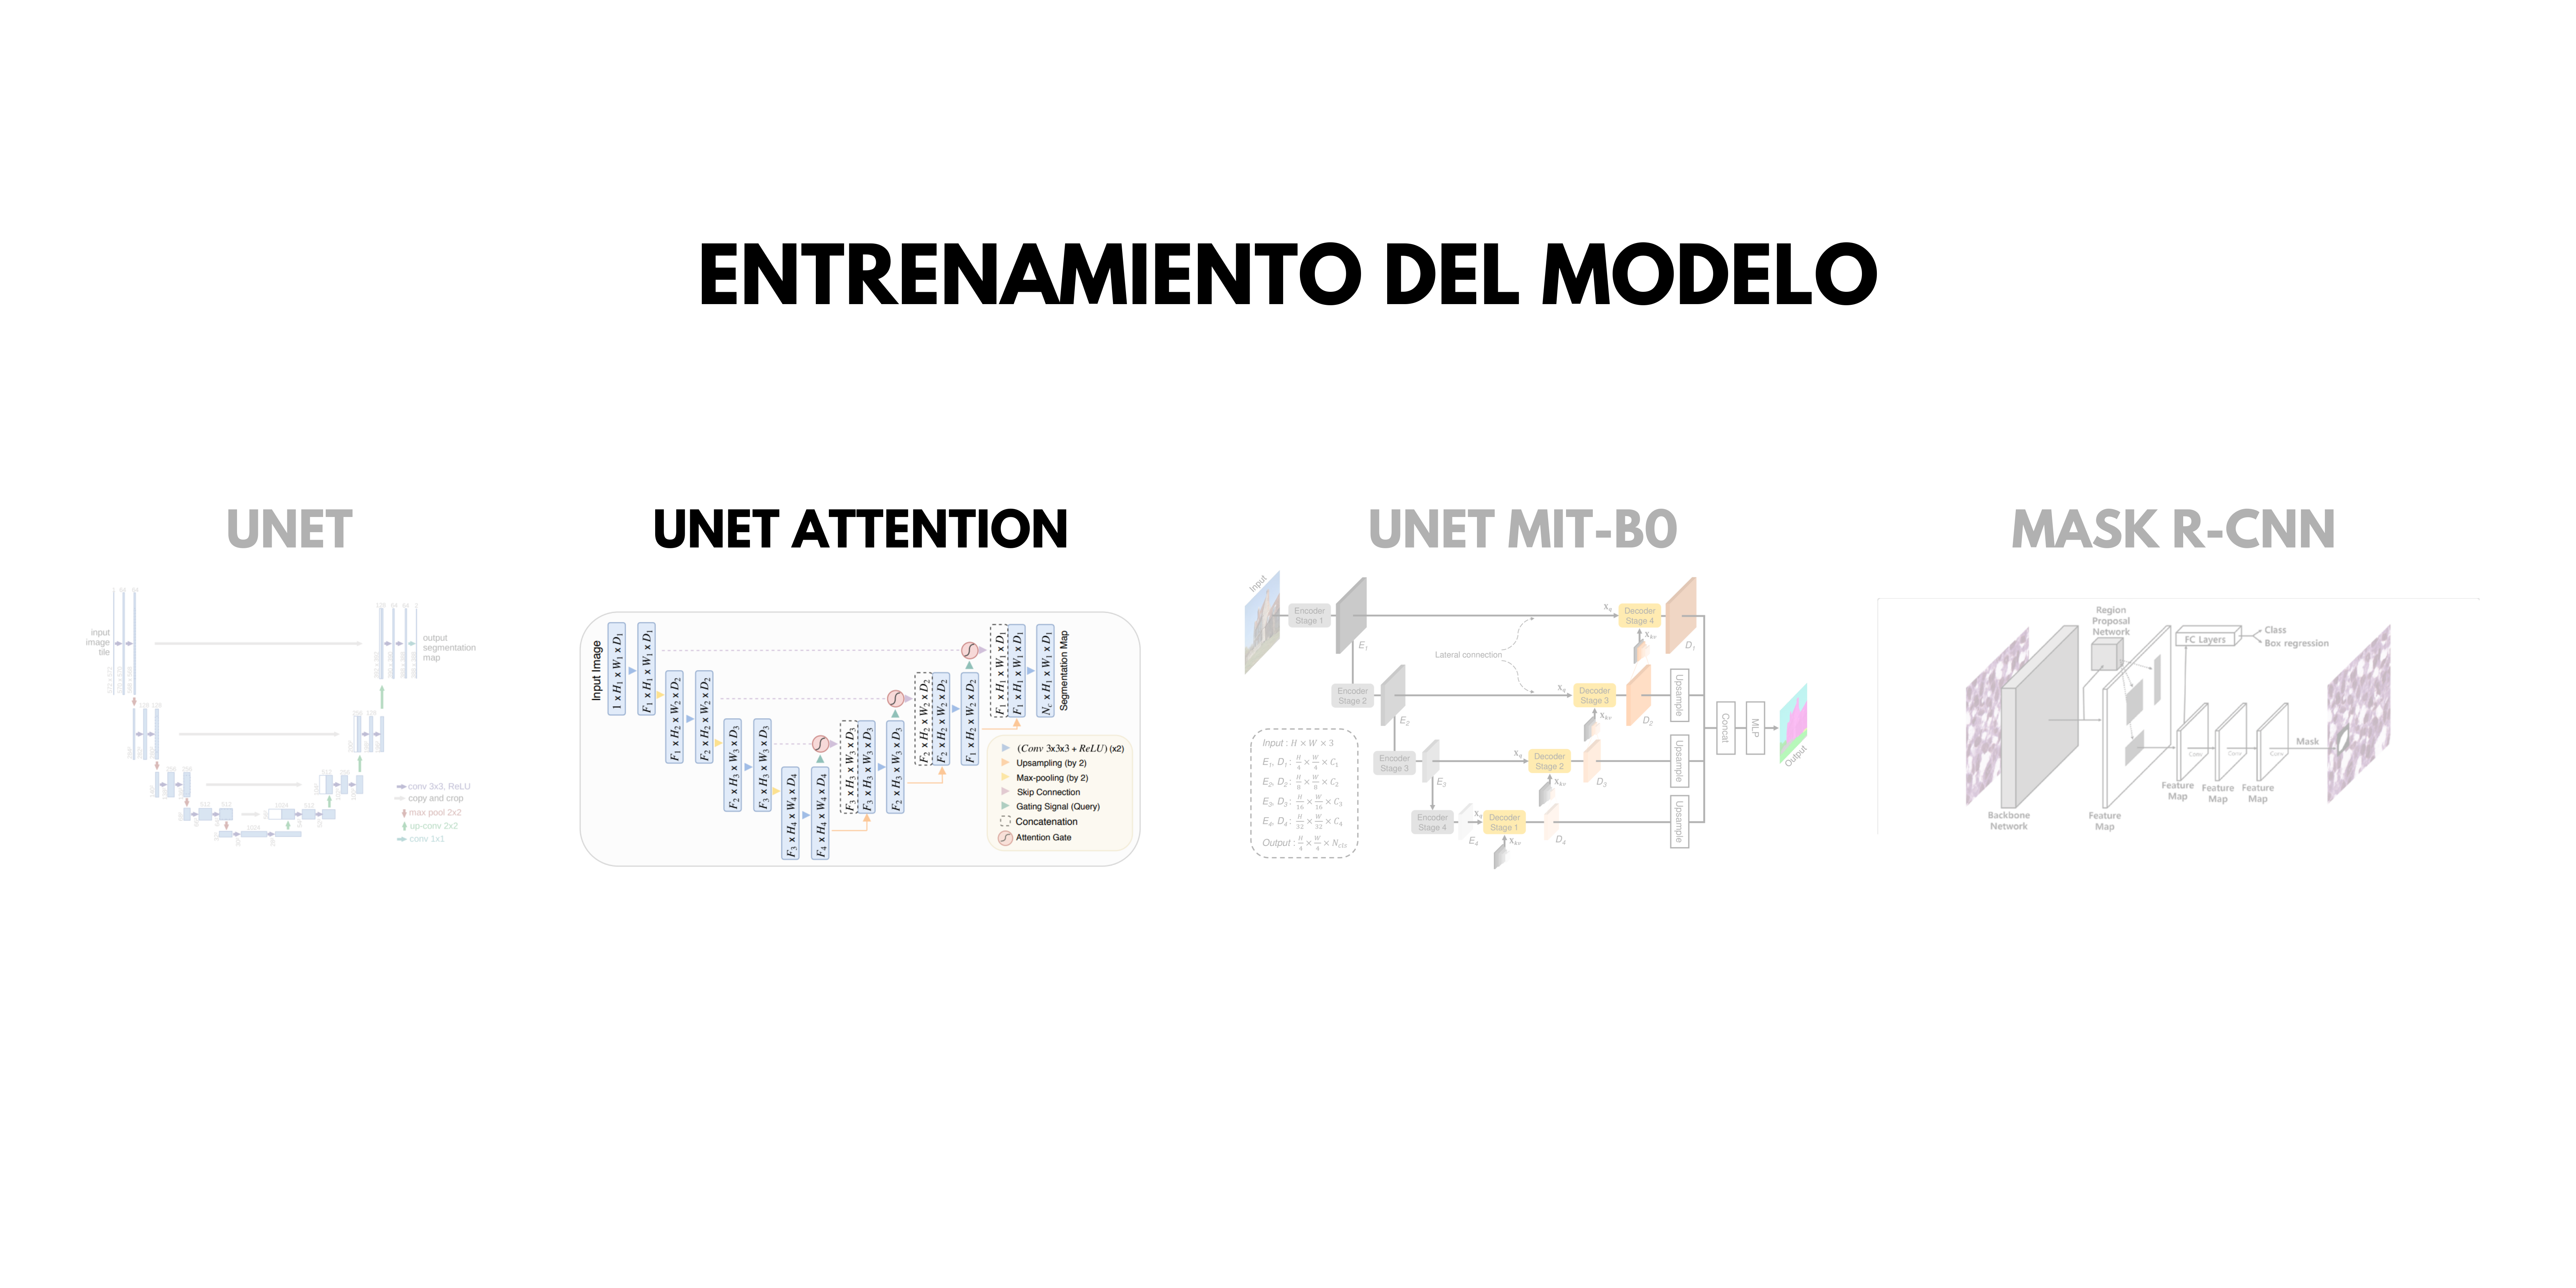
\includegraphics[width=1\textwidth]{4/figures/entrunetat.png}
		\caption[Entrenamiento del Modelo U-Net Attention]{Entrenamiento del Modelo U-Net Attention.\\
		Fuente: Elaboración propia}
		\label{4:figentunetat}
	\end{center}
\end{figure}
  \begin{itemize}
  \item\textbf{Actividad 1 de “\textit{Entrenamiento del modelo}”: Configuración del entorno de entrenamiento}
\\
  Se usó Python 3.10 con PyTorch 2.0.0, Albumentations, OpenCV y CUDA/cuDNN para GPU. Los datos se organizan en carpetas para imágenes y máscaras. El dataset personalizado aplica las transformaciones y divide los datos en 80\% entrenamiento y 20\% validación.

  \item\textbf{Actividad 2 de “\textit{Entrenamiento del modelo}”: Aplicación de técnicas de optimización}
\\  
  Con el objetivo de mejorar la generalización y eficiencia del modelo, se incorporaron varias técnicas de optimización:

\begin{itemize}
  \item \textbf{A.HorizontalFlip(p=0.5)}: aplica volteo horizontal aleatorio con probabilidad 50\%.
  \item \textbf{A.VerticalFlip(p=0.1)}: aplica volteo vertical aleatorio con probabilidad 10\%.
  \item \textbf{A.RandomRotate90(p=0.2)}: rota la imagen aleatoriamente en múltiplos de 90 grados.
  \item \textbf{A.Rotate(limit=15, p=0.3)}: rota la imagen aleatoriamente hasta 15 grados.
  \item \textbf{A.ElasticTransform(alpha=1, sigma=50, approximate=True, p=0.2)}: aplica transformaciones elásticas para simular deformaciones.
  \item \textbf{A.Affine(scale=(0.9, 1.1), translate\_percent=(0.05, 0.05), rotate=(-10, 10), p=0.3)}: realiza escalado, traslación y rotación aleatoria.
  \item \textbf{A.RandomBrightnessContrast(brightness\_limit=0.2, contrast\_limit=0.2, p=0.3)}: modifica aleatoriamente el brillo y contraste.
  \item \textbf{A.GaussNoise(std\_range=(0.2, 0.44), mean\_range=(0, 0), p=0.2)}: añade ruido gaussiano con desviación estándar variable.
  \item \textbf{A.MotionBlur(blur\_limit=3, p=0.1)}: aplica desenfoque de movimiento.
  \item \textbf{A.HueSaturationValue(hue\_shift\_limit=10, sat\_shift\_limit=15, val\_shift\_limit=10, p=0.2)}: ajusta aleatoriamente el tono, la saturación y el valor.
  \item \textbf{A.Resize(256, 256)}: redimensiona la imagen a 256x256 píxeles.
  \item \textbf{ToTensorV2()} : convierte la imagen y máscara en tensores para PyTorch.
  \item \textbf{Entrenamiento:} 50 épocas, batch size 4, con cálculo iterativo de predicción, pérdida, retropropagación y optimización.
  \item \textbf{Tiempo total de entrenamiento:} poco más de una hora y media.
\end{itemize}


  \item\textbf{Actividad 3 de “\textit{Entrenamiento del modelo}”: Validación cruzada del rendimiento}
\\  
  Se usó una partición hold-out (80\% entrenamiento, 20\% validación) para evaluar la capacidad de generalización con métricas como precisión por clase, IoU e índice Dice, garantizando una evaluación rigurosa para imágenes no vistas.

  \end{itemize}
\newpage
  \item \textbf{Modelo de Segmentación: U-Net con codificador MiT-B0 (Mix Transformer)}
  \begin{figure}[H]
	\begin{center}
		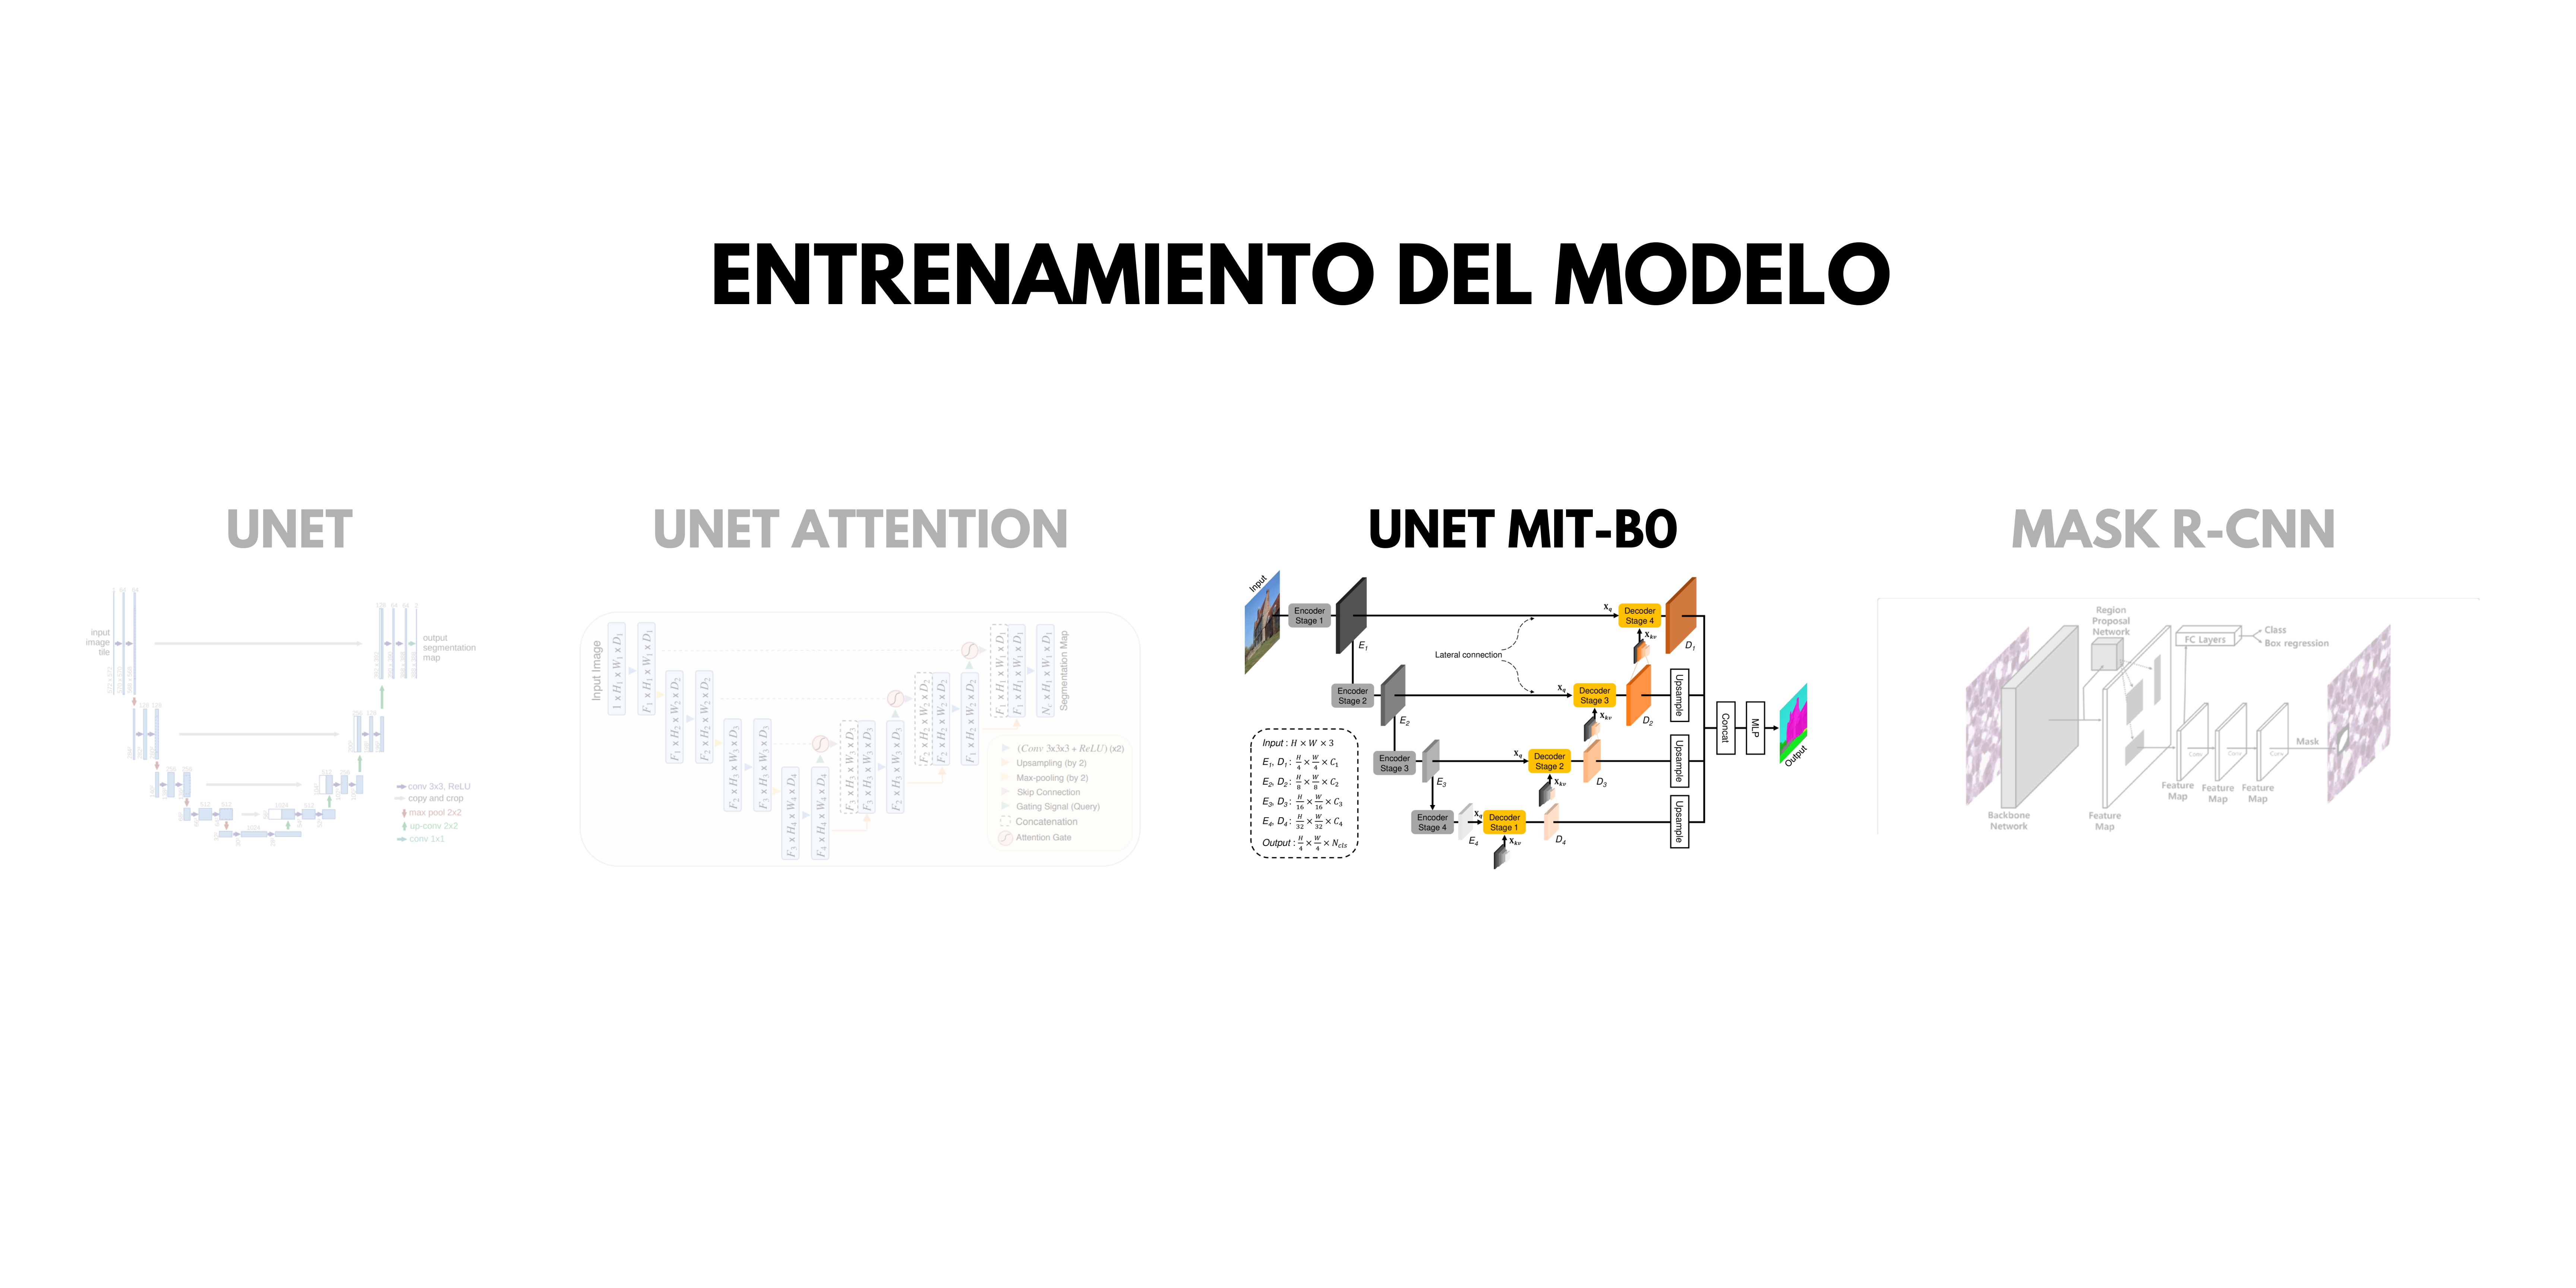
\includegraphics[width=1\textwidth]{4/figures/entrunetmit.png}
		\caption[Entrenamiento del Modelo U-Net con codificador MiT-B0]{Entrenamiento del Modelo U-Net con codificador MiT-B0.\\
		Fuente: Elaboración propia}
		\label{4:figentunetmit}
	\end{center}
\end{figure}
  \begin{itemize}
  \item\textbf{Actividad 1 de “\textit{Entrenamiento del modelo}”: Configuración del entorno de entrenamiento}
\\  
  Se usó Python 3.10 con PyTorch 2.0.0, Albumentations, OpenCV, NumPy y CUDA/cuDNN para GPU. Los datos se organizan en carpetas para imágenes y máscaras. El dataset personalizado aplica las transformaciones y divide los datos en 80\% entrenamiento y 20\% validación.


  \item\textbf{Actividad 2 de “\textit{Entrenamiento del modelo}”: Aplicación de técnicas de optimización}
\\   
  Durante el entrenamiento de la red U-Net con codificador MiT-B0, se implementaron diversas técnicas para mejorar la precisión y velocidad de convergencia del modelo.

\begin{itemize}
\item \textbf{Pesos de clase:} Se calcularon pesos inversamente proporcionales a la frecuencia de cada clase.

\item \textbf{Función de pérdida:} Entropía cruzada ponderada para balancear clases con pesos específicos [0.5, 5.0, 3.0].

\item \textbf{Optimizador:} Adam con tasa de aprendizaje 0.001.

\item \textbf{Entrenamiento:} 50 épocas, batch size 4, con cálculo iterativo de predicción, pérdida, retropropagación y optimización.

\item \textbf{Tiempo total de entrenamiento:} poco más de dos horas.

  \end{itemize}
  

  \item\textbf{Actividad 3 de de “\textit{Entrenamiento del modelo}”: Validación cruzada del rendimiento}
 \\ 
  Se usó una partición hold-out (80\% entrenamiento, 20\% validación) para evaluar la capacidad de generalización con métricas como precisión por clase, IoU e índice Dice, garantizando una evaluación rigurosa para imágenes no vistas.

  \end{itemize}
\newpage
\item \textbf{Modelo de Segmentación: Mask R-CNN}
\begin{figure}[H]
	\begin{center}
		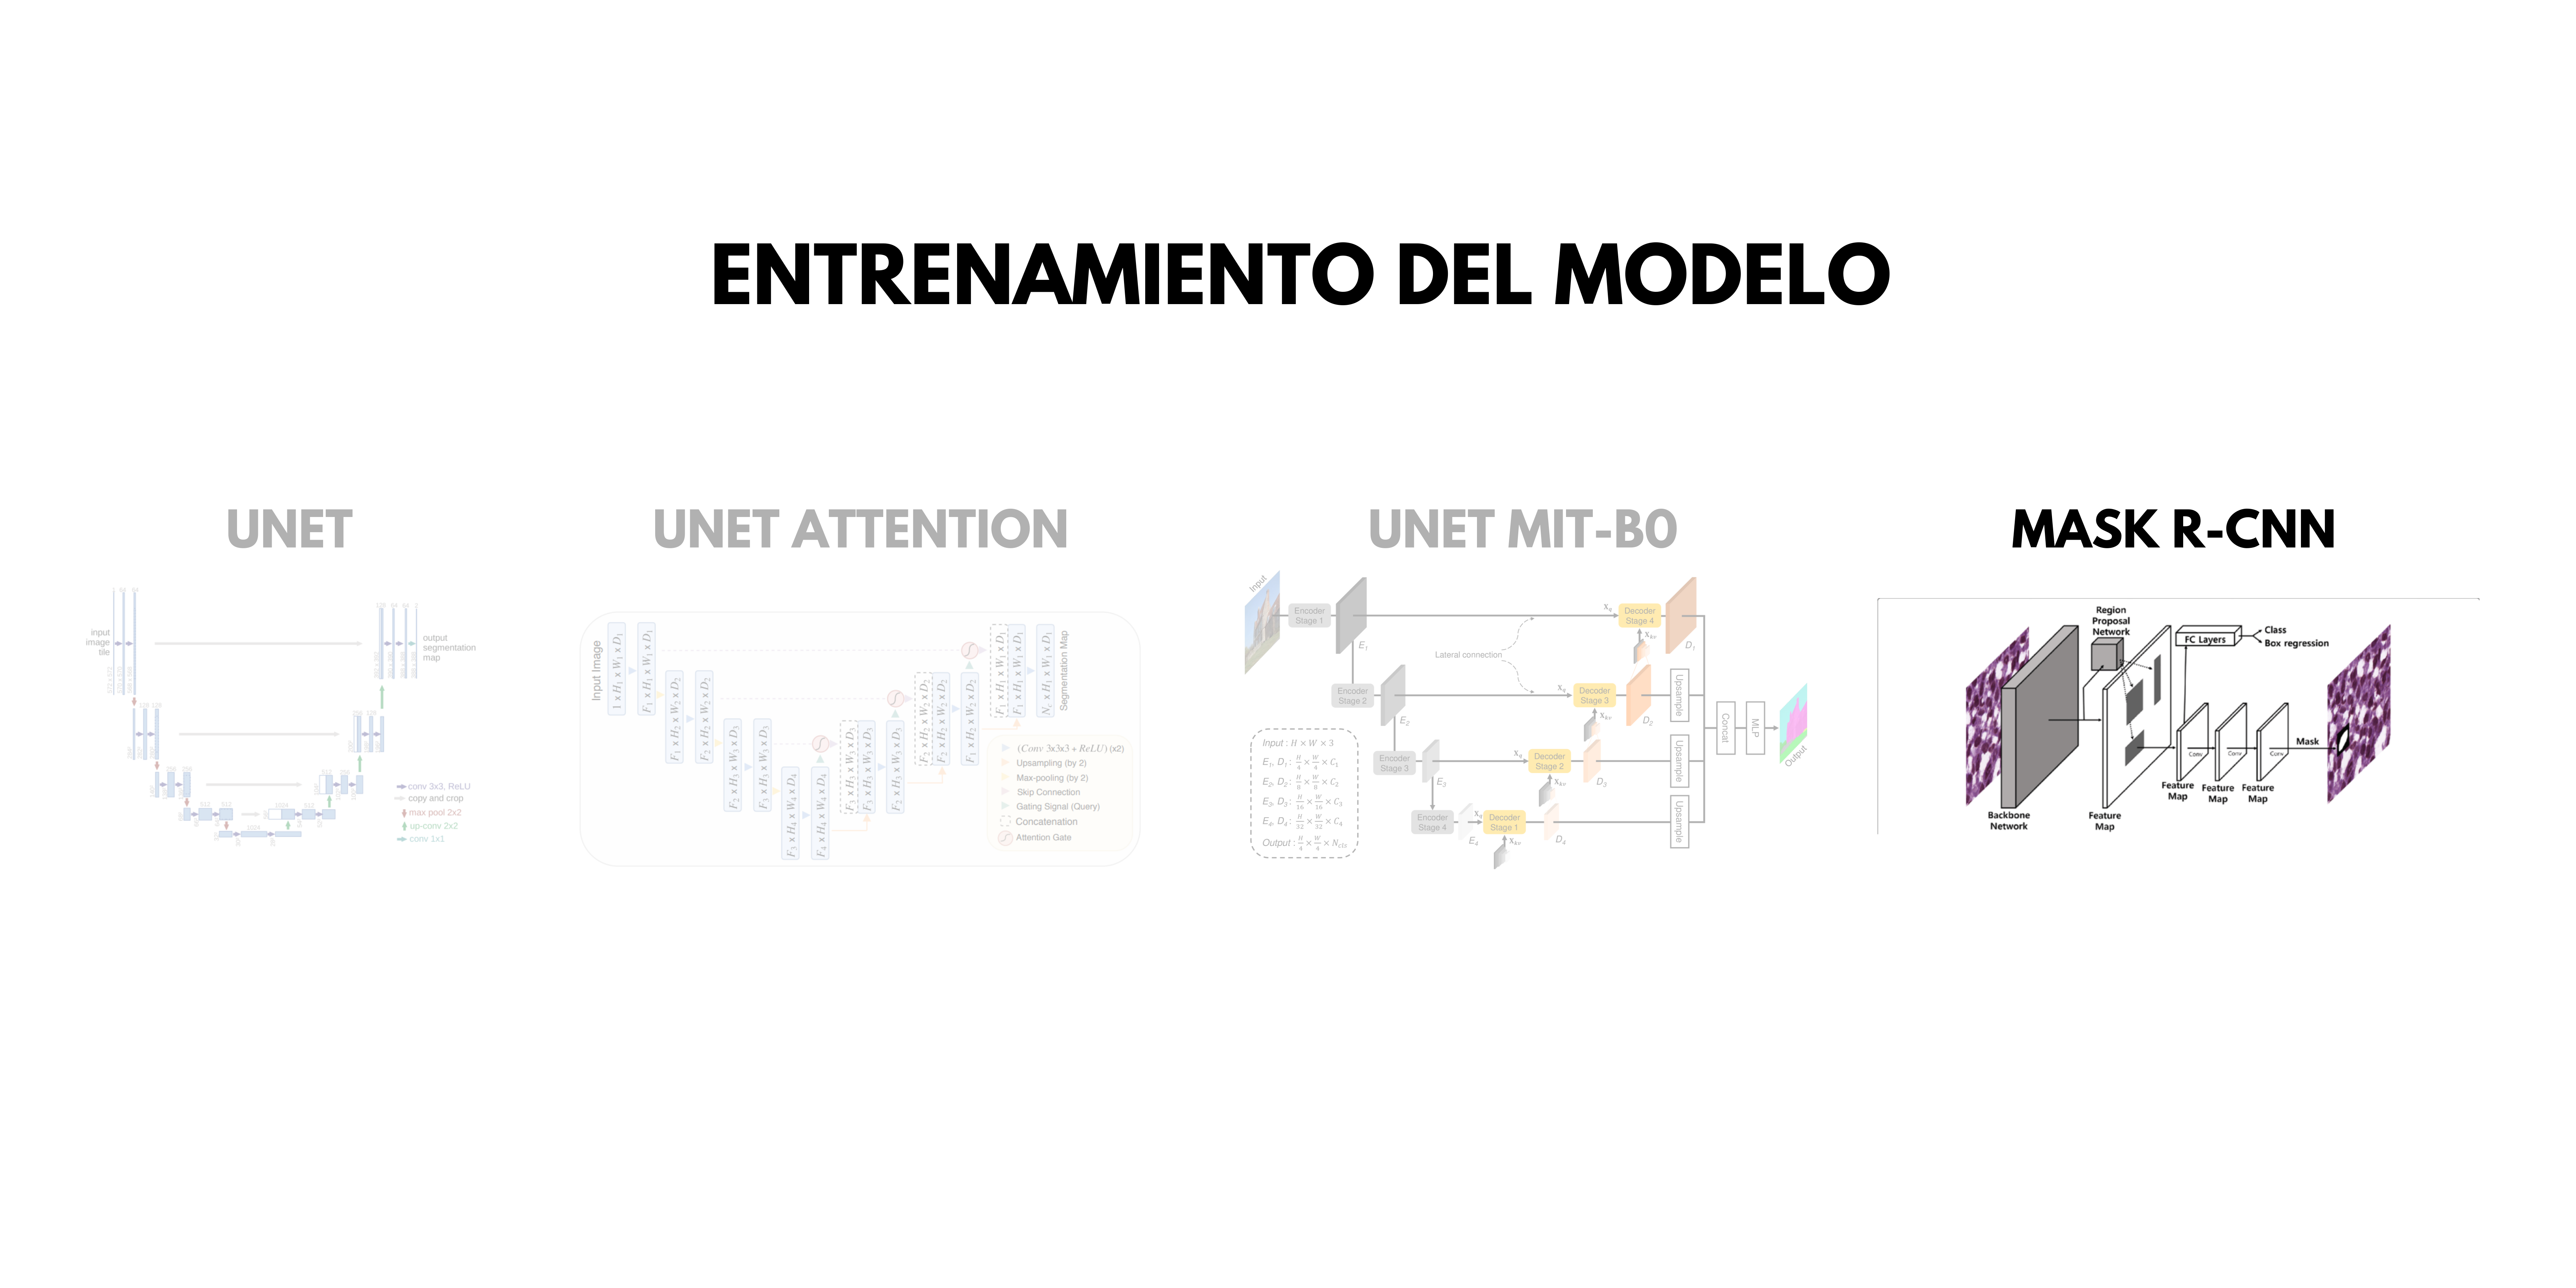
\includegraphics[width=1\textwidth]{4/figures/entrmask.png}
		\caption[Entrenamiento del Modelo Mask R-CNN]{Entrenamiento del Modelo Mask R-CNN.\\
		Fuente: Elaboración propia}
		\label{4:figentmask}
	\end{center}
\end{figure}
  \begin{itemize}
    \item \textbf{Actividad 1 de “\textit{Entrenamiento del modelo}”: Configuración del entorno de entrenamiento}
  \\ 
    Se usó Python 3.10 con PyTorch 2.0.0, Albumentations, OpenCV, NumPy y CUDA/cuDNN para GPU. Los datos se organizan en carpetas para imágenes y máscaras. El dataset personalizado aplica las transformaciones y divide los datos en 80\% entrenamiento y 20\% validación.


  
    \item \textbf{Actividad 2 de “\textit{Entrenamiento del modelo}”: Aplicación de técnicas de optimización}
   \\  
    Con el objetivo de mejorar la generalización y eficiencia del modelo, se incorporaron varias técnicas de optimización:
    
    \begin{itemize}
\item \textbf{Modelo base:} Adaptación del Box Head y Mask Head a 3 clases.

\item \textbf{Optimizador:} Adam con tasa de aprendizaje 0.001.

\item \textbf{Entrenamiento:} 50 épocas, batch size 4, con cálculo iterativo de predicción, pérdida, retropropagación y optimización.

\item \textbf{Tiempo total de entrenamiento:} tres horas.

  \end{itemize}
  
    \item \textbf{Actividad 3 de “\textit{Entrenamiento del modelo}”: Validación cruzada del rendimiento}
   \\ 
    Se usó una partición hold-out (80\% entrenamiento, 20\% validación) para evaluar la capacidad de generalización con métricas como precisión por clase, IoU e índice Dice, garantizando una evaluación rigurosa para imágenes no vistas.

  
  \end{itemize}

\end{enumerate}

\clearpage
\newpage
\section{Evaluación del modelo}

\begin{enumerate}
  \item \textbf{Modelo de Segmentación: U-Net}
  \begin{figure}[H]
	\begin{center}
		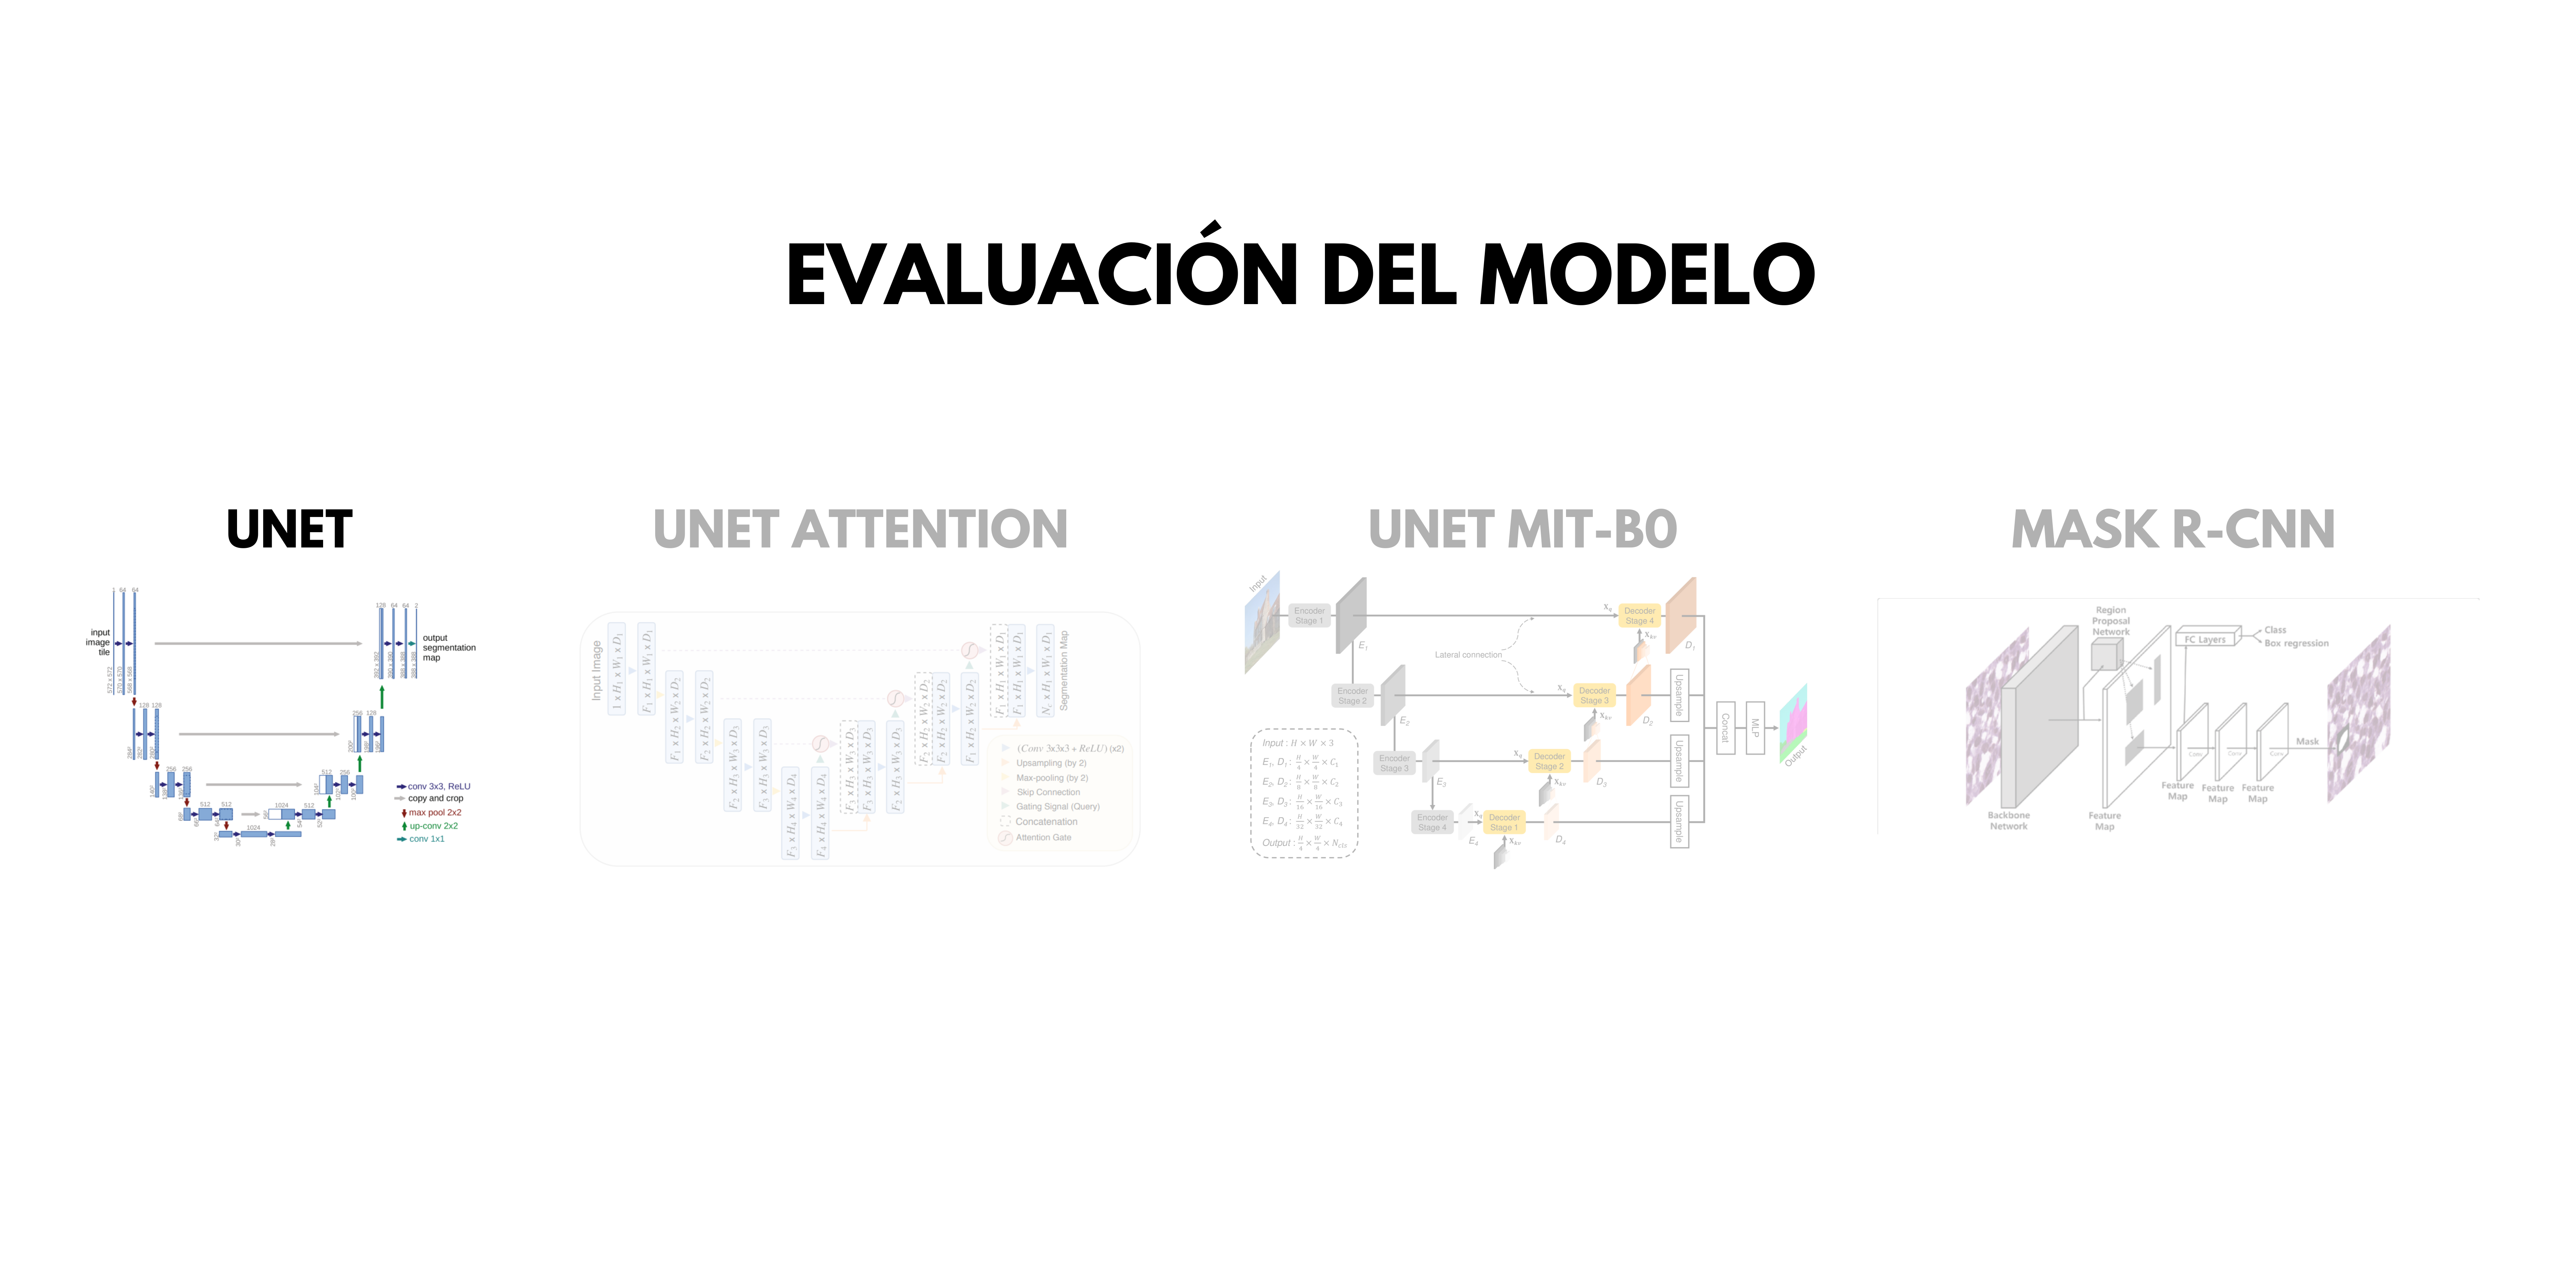
\includegraphics[width=1\textwidth]{4/figures/evunet.png}
		\caption[Evaluación del U-Net]{Evaluación del U-Net.\\
		Fuente: Elaboración propia}
		\label{4:figevunet}
	\end{center}
\end{figure}

  \begin{itemize}
  \item\textbf{Actividad 1 de “\textit{Evaluación del modelo}”: Preparación de Datos de Validación}
  \\
  Como se mencionó antes, se reservó el 20\% de datos para validación con imágenes no vistas durante el entrenamiento, asegurando una estimación imparcial del rendimiento.
  
  \item\textbf{Actividad 2 de “\textit{Evaluación del modelo}”: Definición de Métricas de Evaluación}
  \begin{itemize}
  \item \textbf{Precisión por clase:} Proporción de píxeles que han sido correctamente clasificados para cada clase individual.

  \item \textbf{IoU (Intersection over Union):} El IoU para una clase $c$, denotado como $\text{IoU}_c$, se calcula mediante la siguiente fórmula:
$$\text{IoU}_c = \frac{|P_c \cap G_c|}{|P_c \cup G_c|}$$
donde $P_c$ representa el conjunto de píxeles predichos como pertenecientes a la clase $c$, y $G_c$ representa el conjunto de píxeles que realmente pertenecen a la clase $c$ (ground truth).

  \item \textbf{Coeficiente Dice:} El coeficiente Dice para una clase $c$, denotado como $\text{Dice}_c$, se calcula mediante la siguiente fórmula:
$$\text{Dice}_c = \frac{2|P_c \cap G_c|}{|P_c| + |G_c|}$$
Esta métrica mide el grado de superposición entre la segmentación predicha ($P_c$) y la segmentación verdadera ($G_c$) para la clase $c$.
 

  \item \textbf{Entropía cruzada:} Es una función de pérdida comúnmente utilizada para tareas de segmentación semántica. Evalúa la discrepancia entre la distribución de probabilidad predicha por el modelo y la distribución verdadera de las clases. Para una imagen con $N$ píxeles y $C$ clases, se calcula como:
$$\mathcal{L}_{\text{CE}} = -\sum_{i=1}^{N} \sum_{c=1}^{C} y_{i,c} \log(\hat{y}_{i,c})$$
donde $y_{i,c}$ es una variable binaria que indica si el píxel $i$ pertenece a la clase $c$ (1 si pertenece, 0 en caso contrario), y $\hat{y}_{i,c}$ es la probabilidad predicha por el modelo de que el píxel $i$ pertenezca a la clase $c$. Esta función penaliza con mayor intensidad las predicciones incorrectas y es útil cuando se requiere una clasificación pixel a pixel precisa.
\end{itemize}

Estas métricas proporcionan una evaluación integral del desempeño del modelo de segmentación.



  \item\textbf{Actividad 3 de “\textit{Evaluación del modelo}”: Evaluación del Modelo}
  \begin{itemize}
    \item \textbf{Resultados:}\\
El modelo alcanzó los siguientes resultados promedio sobre el conjunto de validación:
\begin{itemize}
  \item \textbf{Pérdida mínima (\texttt{val\_loss}):} 0.1849 
  \item \textbf{Precisión promedio:} 0.832, indicando que la mayoría de los píxeles se clasificaron correctamente.
  \item \textbf{Dice Score promedio:} 0.712, mostrando un nivel bueno de superposición entre máscaras predichas y reales.
  \item \textbf{Jaccard Index promedio:} 0.759, reflejando buenas coincidencias exactas en regiones complejas.
  \item Se detectaron mejores resultados en la clase \emph{arrugas}, posiblemente por la mayor representación y contraste de textura.
  \item La clase \emph{manchas} presentó métricas ligeramente inferiores, sugiriendo que futuras optimizaciones deberían incluir aumentos más dirigidos a mejorar esta categoría (por ejemplo, resaltando contraste o coloración).
\end{itemize}
  A continuación se presentan las métricas calculadas, los gráficos obtenidos y los ejemplos visuales para ilustrar el rendimiento del modelo en las Figuras \ref{fig:validacion11}, \ref{fig:validacion22} y \ref{fig:validacion33}.

  \vspace{0.2cm}
  \begin{figure}[H]
\centering
\includegraphics[width=0.75\textwidth]{4/figures/UnetComparación1.png}
\caption{Comparación visual: imagen original, máscara real multicategoría y predicción del modelo para un caso con predominio de arrugas.}
\label{fig:validacion11}
\end{figure}

\begin{figure}[H]
\centering
\includegraphics[width=0.75\textwidth]{4/figures/UnetComparación2.png}
\caption{Comparación visual: ejemplo donde se observa el desempeño del modelo en la detección de manchas, destacando regiones correctamente identificadas y algunas áreas faltantes.}
\label{fig:validacion22}
\end{figure}

\begin{figure}[H]
\centering
\includegraphics[width=0.75\textwidth]{4/figures/UnetComparación3.png}
\caption{Comparación visual: caso mixto donde se presentan simultáneamente arrugas y manchas, mostrando la capacidad del modelo para diferenciar ambas clases en un mismo rostro.}
\label{fig:validacion33}
\end{figure}
\end{itemize}

  \end{itemize}
  \newpage
  \item \textbf{Modelo de Segmentación: U-Net Attention}
  \begin{figure}[H]
	\begin{center}
		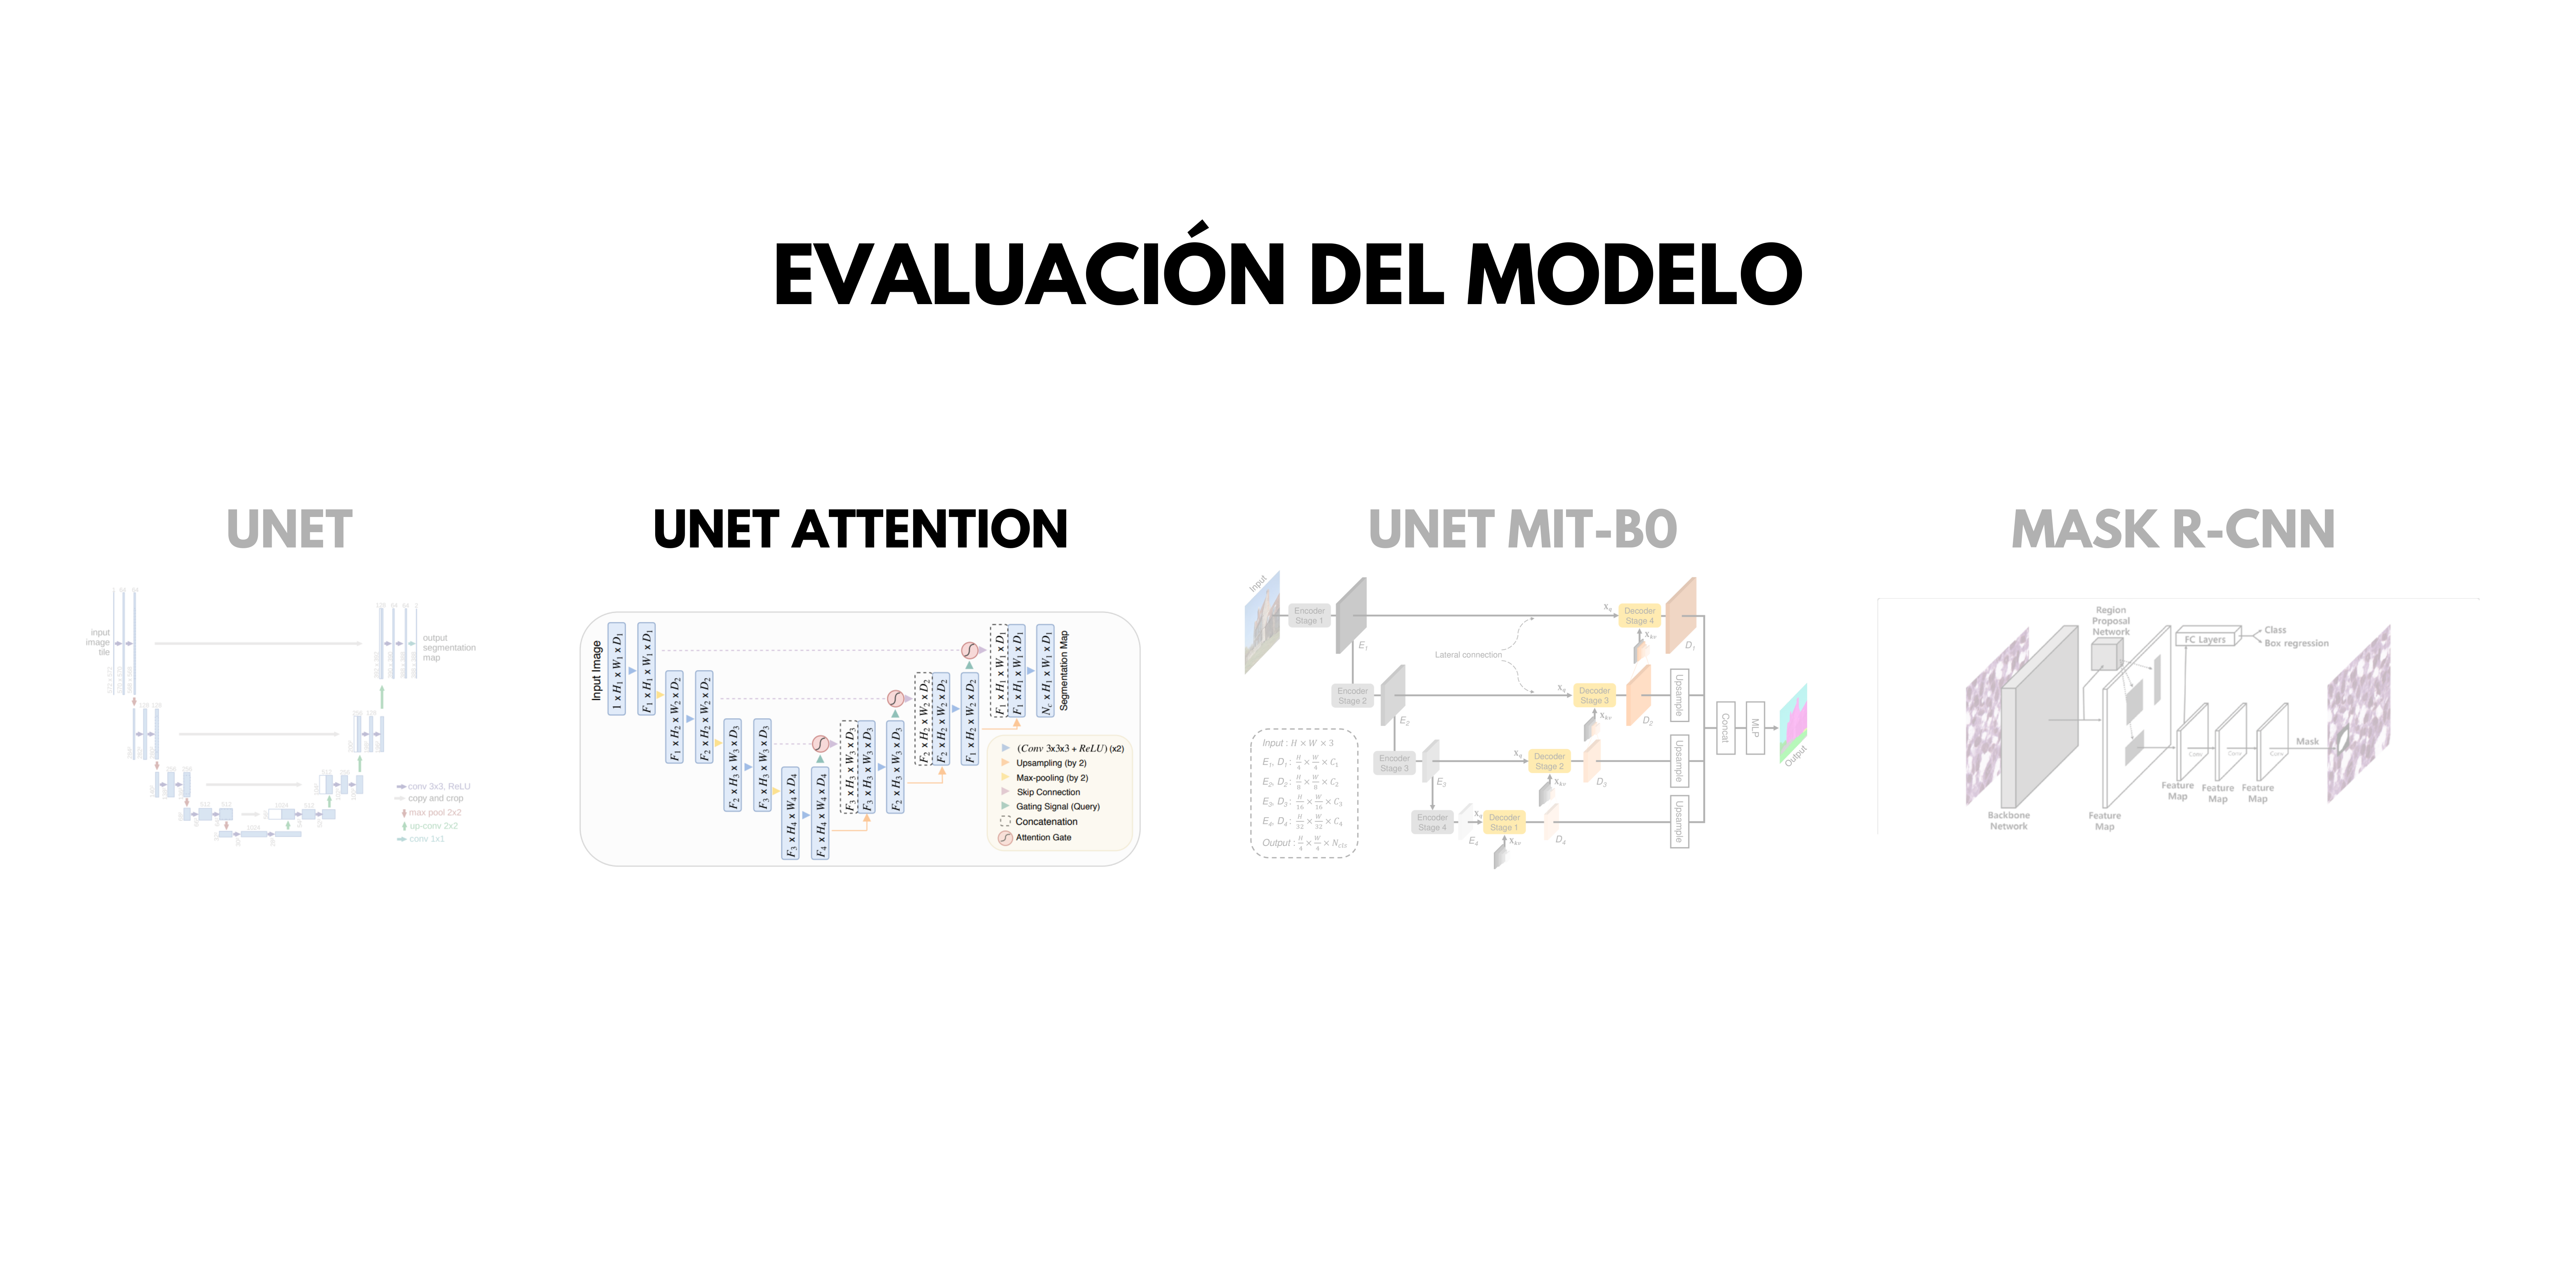
\includegraphics[width=1\textwidth]{4/figures/evunetat.png}
		\caption[Evaluación del U-Net Attention]{Evaluación del U-Net Attention.\\
		Fuente: Elaboración propia}
		\label{4:figevunetat}
	\end{center}
\end{figure}
  \begin{itemize}
  \item\textbf{Actividad 1 de “\textit{Evaluación del modelo}”: Preparación de Datos de Validación}
  \\
  Como se mencionó antes, se reservó el 20\% de datos para validación con imágenes no vistas durante el entrenamiento, asegurando una estimación imparcial del rendimiento.
  

  \item\textbf{Actividad 2 de “\textit{Evaluación del modelo}”: Definición de Métricas de Evaluación}
    \begin{itemize}
  \item \textbf{Precisión por clase:} Proporción de píxeles que han sido correctamente clasificados para cada clase individual.

  \item \textbf{IoU (Intersection over Union):} El IoU para una clase $c$, denotado como $\text{IoU}_c$, se calcula mediante la siguiente fórmula:
$$\text{IoU}_c = \frac{|P_c \cap G_c|}{|P_c \cup G_c|}$$
donde $P_c$ representa el conjunto de píxeles predichos como pertenecientes a la clase $c$, y $G_c$ representa el conjunto de píxeles que realmente pertenecen a la clase $c$ (ground truth).

  \item \textbf{Coeficiente Dice:} El coeficiente Dice para una clase $c$, denotado como $\text{Dice}_c$, se calcula mediante la siguiente fórmula:
$$\text{Dice}_c = \frac{2|P_c \cap G_c|}{|P_c| + |G_c|}$$
Esta métrica mide el grado de superposición entre la segmentación predicha ($P_c$) y la segmentación verdadera ($G_c$) para la clase $c$.
 

  \item \textbf{Entropía cruzada:} Es una función de pérdida comúnmente utilizada para tareas de segmentación semántica. Evalúa la discrepancia entre la distribución de probabilidad predicha por el modelo y la distribución verdadera de las clases. Para una imagen con $N$ píxeles y $C$ clases, se calcula como:
$$\mathcal{L}_{\text{CE}} = -\sum_{i=1}^{N} \sum_{c=1}^{C} y_{i,c} \log(\hat{y}_{i,c})$$
donde $y_{i,c}$ es una variable binaria que indica si el píxel $i$ pertenece a la clase $c$ (1 si pertenece, 0 en caso contrario), y $\hat{y}_{i,c}$ es la probabilidad predicha por el modelo de que el píxel $i$ pertenezca a la clase $c$. Esta función penaliza con mayor intensidad las predicciones incorrectas y es útil cuando se requiere una clasificación pixel a pixel precisa.
\end{itemize}

Estas métricas proporcionan una evaluación integral del desempeño del modelo de segmentación.


  \item\textbf{Actividad 3 de “\textit{Evaluación del modelo}”: Evaluación del Modelo}
  El modelo alcanzó los siguientes resultados promedio sobre el conjunto de validación:
\begin{itemize}
  \item \textbf{Pérdida mínima (\texttt{val\_loss}):} 0.1158
  \item \textbf{Precisión promedio:} 0.911, indicando que gran parte de los píxeles se clasificaron correctamente.
  \item \textbf{Dice Score promedio:} 0.810, mostrando un nivel superior de superposición entre máscaras predichas y reales.
  \item \textbf{Jaccard Index promedio:} 0.852, reflejando buenas coincidencias exactas en regiones complejas.
  \item Se detectaron mejores resultados en la clase \emph{arrugas}, posiblemente por la mayor representación y contraste de textura.
  \item La clase \emph{manchas} presentó métricas ligeramente inferiores, sugiriendo que futuras optimizaciones deberían incluir aumentos más dirigidos a mejorar esta categoría (por ejemplo, resaltando contraste o coloración).
\end{itemize}

\vspace{0.5cm}

Además de los resultados numéricos, se generaron visualizaciones comparativas entre los datos reales y las predicciones del modelo. Estas imágenes permiten evaluar cualitativamente el desempeño del modelo, mostrando tanto los aciertos como las áreas de mejora. A continuación, se presentan, en las Figuras \ref{fig:validacion1}, \ref{fig:validacion2} y \ref{fig:validacion3}, tres ejemplos destacados:

\vspace{0.5cm}

\begin{figure}[H]
\centering
\includegraphics[width=0.75\textwidth]{4/figures/comparación9.png}
\caption{Comparación visual: imagen original, máscara real multicategoría y predicción del modelo para un caso con predominio de arrugas.}
\label{fig:validacion1}
\end{figure}

\begin{figure}[H]
\centering
\includegraphics[width=0.75\textwidth]{4/figures/comparación6.png}
\caption{Comparación visual: ejemplo donde se observa el desempeño del modelo en la detección de manchas, destacando regiones correctamente identificadas y algunas áreas faltantes.}
\label{fig:validacion2}
\end{figure}

\begin{figure}[H]
\centering
\includegraphics[width=0.75\textwidth]{4/figures/comparación1.png}
\caption{Comparación visual: caso mixto donde se presentan simultáneamente arrugas y manchas, mostrando la capacidad del modelo para diferenciar ambas clases en un mismo rostro.}
\label{fig:validacion3}
\end{figure}

  \end{itemize}

  \newpage
  \item \textbf{Modelo de Segmentación: U-Net con codificador MiT-B0 (Mix Transformer)}
  \begin{figure}[H]
	\begin{center}
		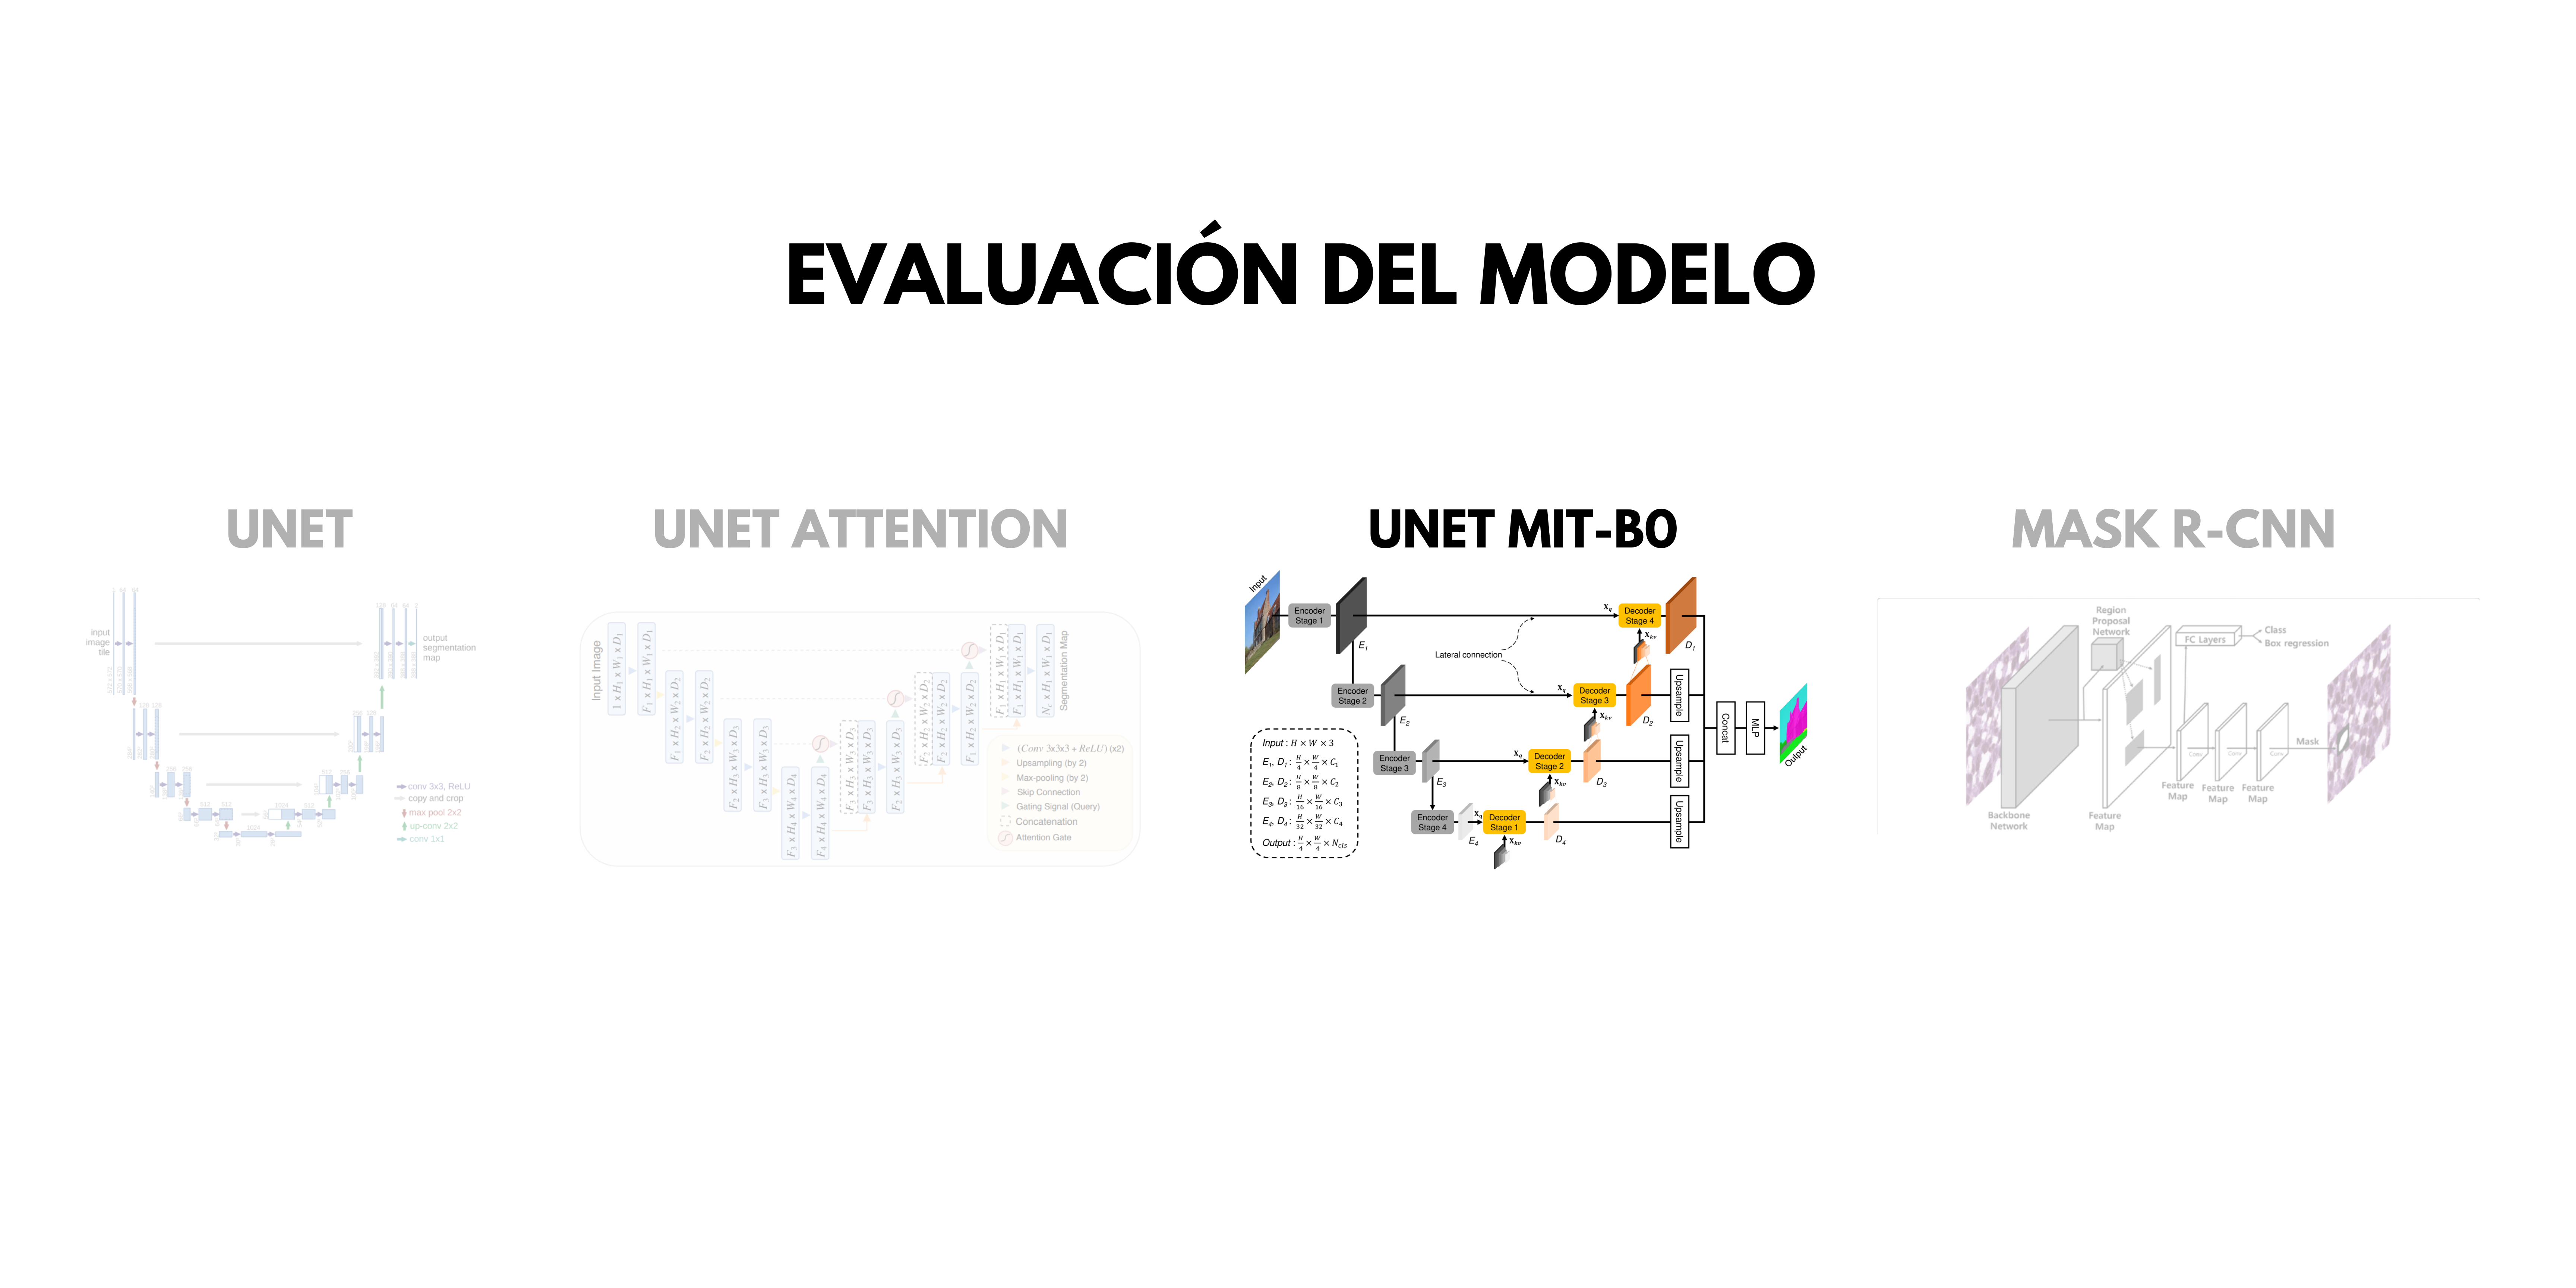
\includegraphics[width=1\textwidth]{4/figures/evunetmit.png}
		\caption[Evaluación del U-Net con codificador MiT-B0]{Evaluación del U-Net con codificador MiT-B0.\\
		Fuente: Elaboración propia}
		\label{4:figevunetmit}
	\end{center}
\end{figure}
  \begin{itemize}
  \item\textbf{Actividad 1 de “\textit{Evaluación del modelo}”: Preparación de Datos de Validación}
  \\
  Como se mencionó antes, se reservó el 20\% de datos para validación con imágenes no vistas durante el entrenamiento, asegurando una estimación imparcial del rendimiento.
  
  \item\textbf{Actividad 2 de “\textit{Evaluación del modelo}”: Definición de Métricas de Evaluación}
     \begin{itemize}
  \item \textbf{Precisión por clase:} Proporción de píxeles que han sido correctamente clasificados para cada clase individual.

  \item \textbf{IoU (Intersection over Union):} El IoU para una clase $c$, denotado como $\text{IoU}_c$, se calcula mediante la siguiente fórmula:
$$\text{IoU}_c = \frac{|P_c \cap G_c|}{|P_c \cup G_c|}$$
donde $P_c$ representa el conjunto de píxeles predichos como pertenecientes a la clase $c$, y $G_c$ representa el conjunto de píxeles que realmente pertenecen a la clase $c$ (ground truth).

  \item \textbf{Coeficiente Dice:} El coeficiente Dice para una clase $c$, denotado como $\text{Dice}_c$, se calcula mediante la siguiente fórmula:
$$\text{Dice}_c = \frac{2|P_c \cap G_c|}{|P_c| + |G_c|}$$
Esta métrica mide el grado de superposición entre la segmentación predicha ($P_c$) y la segmentación verdadera ($G_c$) para la clase $c$.
 

  \item \textbf{Entropía cruzada:} Es una función de pérdida comúnmente utilizada para tareas de segmentación semántica. Evalúa la discrepancia entre la distribución de probabilidad predicha por el modelo y la distribución verdadera de las clases. Para una imagen con $N$ píxeles y $C$ clases, se calcula como:
$$\mathcal{L}_{\text{CE}} = -\sum_{i=1}^{N} \sum_{c=1}^{C} y_{i,c} \log(\hat{y}_{i,c})$$
donde $y_{i,c}$ es una variable binaria que indica si el píxel $i$ pertenece a la clase $c$ (1 si pertenece, 0 en caso contrario), y $\hat{y}_{i,c}$ es la probabilidad predicha por el modelo de que el píxel $i$ pertenezca a la clase $c$. Esta función penaliza con mayor intensidad las predicciones incorrectas y es útil cuando se requiere una clasificación pixel a pixel precisa.
\end{itemize}

Estas métricas proporcionan una evaluación integral del desempeño del modelo de segmentación.



  \item\textbf{Actividad 3 de “\textit{Evaluación del modelo}”: Evaluación del Modelo}
  \\
  El modelo entrenado alcanzó un rendimiento destacable en comparación con la versión original de U-Net. Los resultados promedio sobre el conjunto de validación fueron:

\begin{itemize}
\item \textbf{Pérdida mínima (\texttt{val\_loss}):} 0.0441.
\item \textbf{Precisión promedio:} 0.771.
\item \textbf{Dice Score promedio:} 0.563.
\item \textbf{IoU promedio:} 0.647.
\item La clase \emph{manchas} mostró mejoras claras en comparación con el modelo base, alcanzando un Dice de 0.881 frente a 0.852.
\item La clase \emph{arrugas} también mostró una segmentación más limpia y continua.

\end{itemize}
Estas métricas confirman que la integración del codificador MiT-B0 aporta beneficios tangibles, especialmente en la capacidad del modelo para interpretar el contexto global de la imagen.



  Además de los resultados numéricos, se generaron visualizaciones comparativas entre los datos reales y las predicciones del modelo. Estas imágenes permiten evaluar cualitativamente el desempeño del modelo, mostrando tanto los aciertos como las áreas de mejora. A continuación, se presentan, en las Figuras \ref{fig:validacionunetvit1}, \ref{fig:validacionunetvit2} y \ref{fig:validacionunetvit3}, tres ejemplos destacados:

  \vspace{0.5cm}
  
  \begin{figure}[H]
  \centering
  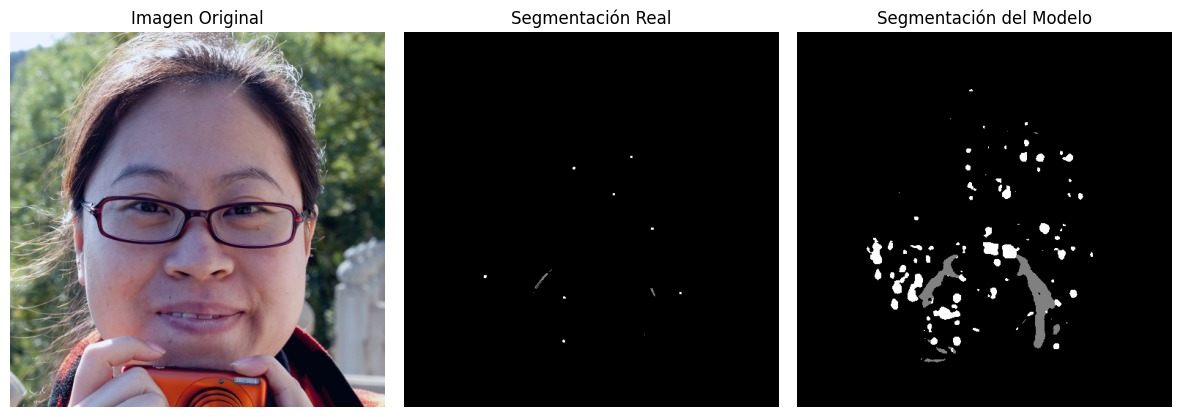
\includegraphics[width=0.75\textwidth]{4/figures/unetvit1.jpg}
  \caption{Comparación visual: imagen original, máscara real multicategoría y predicción del modelo para un caso con predominio de manchas.}
  \label{fig:validacionunetvit1}
  \end{figure}
  
  \begin{figure}[H]
  \centering
  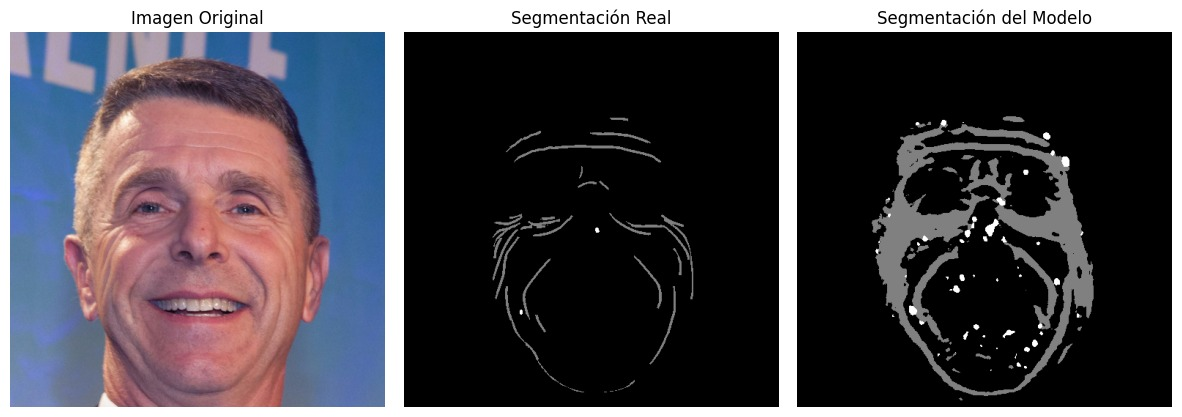
\includegraphics[width=0.75\textwidth]{4/figures/unetvit2.jpg}
  \caption{Comparación visual: ejemplo donde se observa el desempeño del modelo en la detección de manchas, destacando pocas regiones correctamente identificadas y la mayoría de áreas faltantes.}
  \label{fig:validacionunetvit2}
  \end{figure}
  
  \begin{figure}[H]
    \centering
    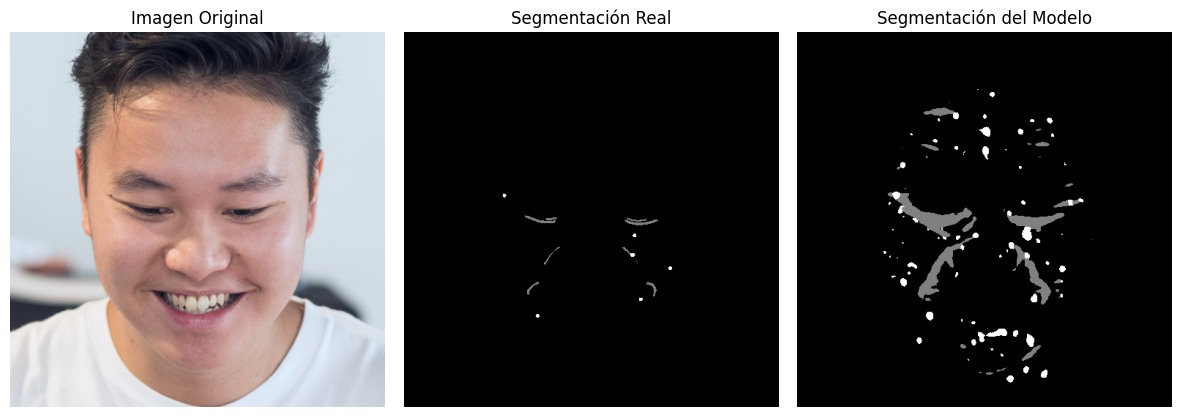
\includegraphics[width=0.75\textwidth]{4/figures/unetvit3.jpg}
    \caption{Comparación visual: ejemplo donde se observa el desempeño del modelo en la detección de manchas, destacando casi ninguna de las regiones correctamente identificadas y muchas áreas faltantes.}
    \label{fig:validacionunetvit3}
    \end{figure}

  \end{itemize}


  \item \textbf{Modelo de Segmentación: Mask R-CNN}
  \begin{figure}[H]
	\begin{center}
		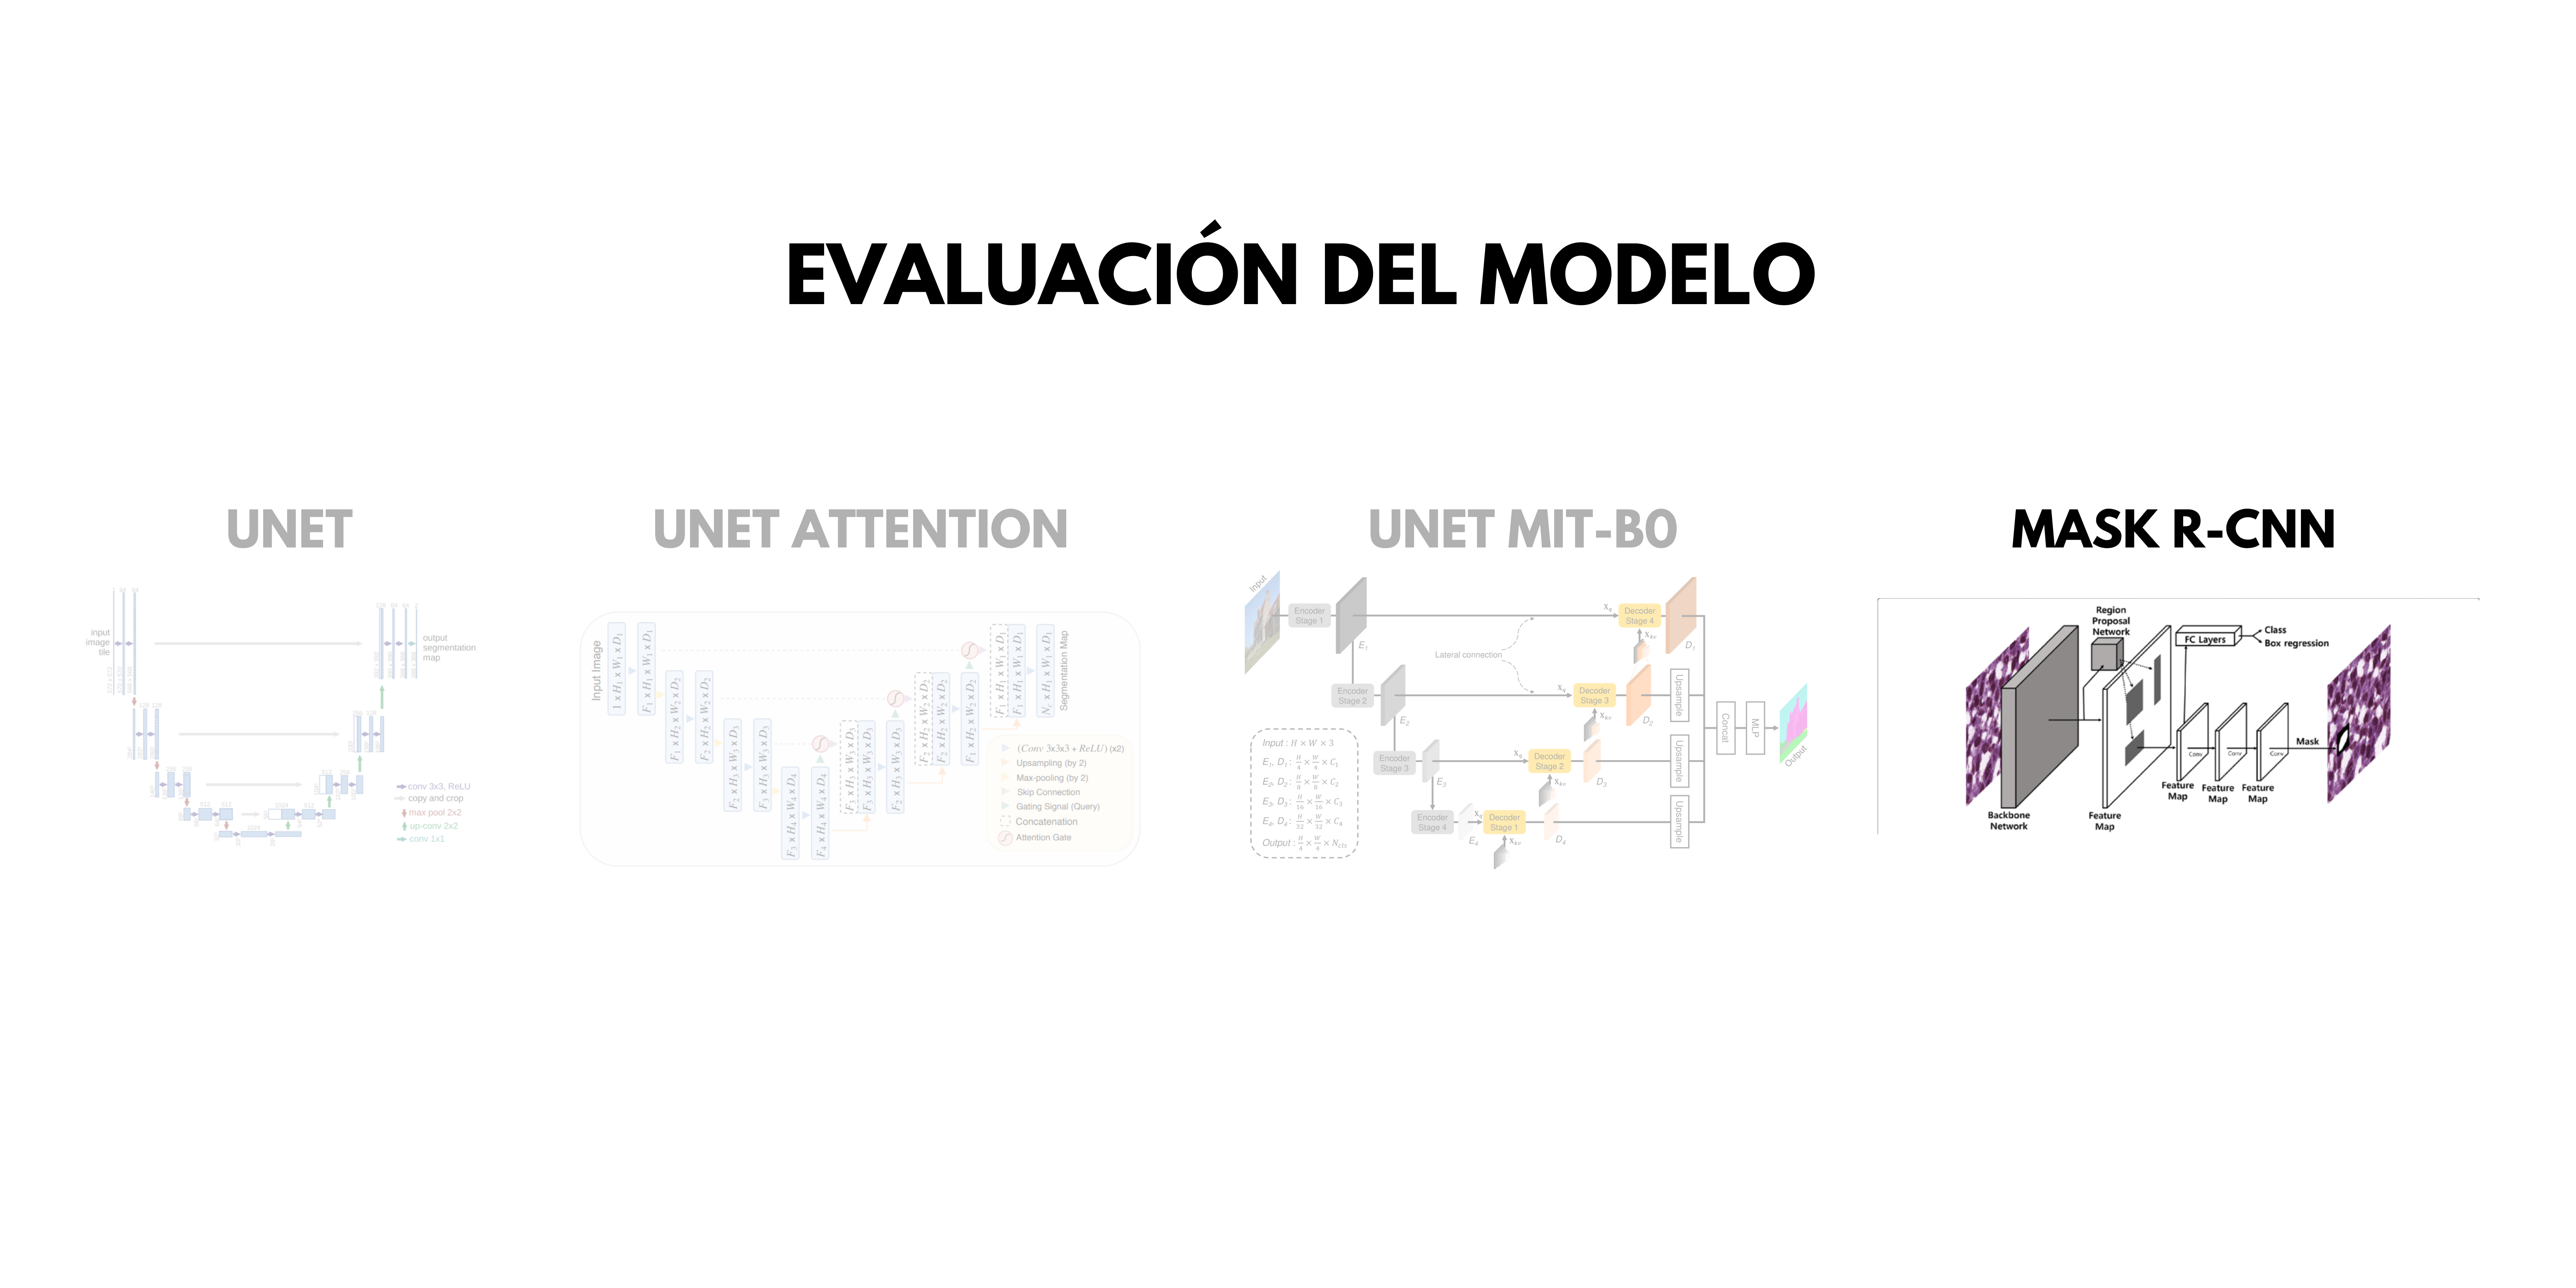
\includegraphics[width=1\textwidth]{4/figures/evmask.png}
		\caption[Evaluación del Mask R-CNN]{Evaluación del Mask R-CNN.\\
		Fuente: Elaboración propia}
		\label{4:figevmask}
	\end{center}
\end{figure}
  \begin{itemize}
  
    \item \textbf{Actividad 1 de “\textit{Evaluación del modelo}”: Preparación de Datos de Validación} \\
    \\
    Como se mencionó antes, se reservó el 20\% de datos para validación con imágenes no vistas durante el entrenamiento, asegurando una estimación imparcial del rendimiento.
  
  
    \item \textbf{Actividad 2 de “\textit{Evaluación del modelo}”: Definición de Métricas de Evaluación}
     \begin{itemize}
  \item \textbf{Precisión por clase:} Proporción de píxeles que han sido correctamente clasificados para cada clase individual.

  \item \textbf{IoU (Intersection over Union):} El IoU para una clase $c$, denotado como $\text{IoU}_c$, se calcula mediante la siguiente fórmula:
$$\text{IoU}_c = \frac{|P_c \cap G_c|}{|P_c \cup G_c|}$$
donde $P_c$ representa el conjunto de píxeles predichos como pertenecientes a la clase $c$, y $G_c$ representa el conjunto de píxeles que realmente pertenecen a la clase $c$ (ground truth).

  \item \textbf{Coeficiente Dice:} El coeficiente Dice para una clase $c$, denotado como $\text{Dice}_c$, se calcula mediante la siguiente fórmula:
$$\text{Dice}_c = \frac{2|P_c \cap G_c|}{|P_c| + |G_c|}$$
Esta métrica mide el grado de superposición entre la segmentación predicha ($P_c$) y la segmentación verdadera ($G_c$) para la clase $c$.
 

  \item \textbf{Entropía cruzada:} Es una función de pérdida comúnmente utilizada para tareas de segmentación semántica. Evalúa la discrepancia entre la distribución de probabilidad predicha por el modelo y la distribución verdadera de las clases. Para una imagen con $N$ píxeles y $C$ clases, se calcula como:
$$\mathcal{L}_{\text{CE}} = -\sum_{i=1}^{N} \sum_{c=1}^{C} y_{i,c} \log(\hat{y}_{i,c})$$
donde $y_{i,c}$ es una variable binaria que indica si el píxel $i$ pertenece a la clase $c$ (1 si pertenece, 0 en caso contrario), y $\hat{y}_{i,c}$ es la probabilidad predicha por el modelo de que el píxel $i$ pertenezca a la clase $c$. Esta función penaliza con mayor intensidad las predicciones incorrectas y es útil cuando se requiere una clasificación pixel a pixel precisa.
\end{itemize}

Estas métricas proporcionan una evaluación integral del desempeño del modelo de segmentación.

    \item \textbf{Actividad 3 de “\textit{Evaluación del modelo}”: Evaluación del Modelo} \\
    \\
    Los resultados del modelo Mask R-CNN sobre el conjunto de validación fueron los siguientes:
    \begin{itemize}
      \item \textbf{Pérdida mínima (\texttt{val\_loss}):} 0.441.
      \item \textbf{Precisión:} 0.153.
      \item \textbf{Dice Score:} 0.052.
      \item \textbf{Jaccard Index (IoU):} 0.221.
      \item La clase \emph{manchas} obtuvo una segmentación nada precisa.
      \item La clase \emph{arrugas} mostró un desempeño muy inferior debido a la dificultad de detección sin bordes claros.
    \end{itemize}
  
    Además de los resultados numéricos, se generaron visualizaciones comparativas entre los datos reales y las predicciones del modelo. Estas imágenes permiten evaluar cualitativamente el desempeño del modelo, mostrando tanto los aciertos como las áreas de mejora. A continuación, se presentan, en las Figuras \ref{fig:validacionmaskrcnn1}, \ref{fig:validacionmaskrcnn2} y \ref{fig:validacionmaskrcnn3}, tres ejemplos destacados:
  
    \vspace{0.5cm}
  
    \begin{figure}[H]
      \centering
      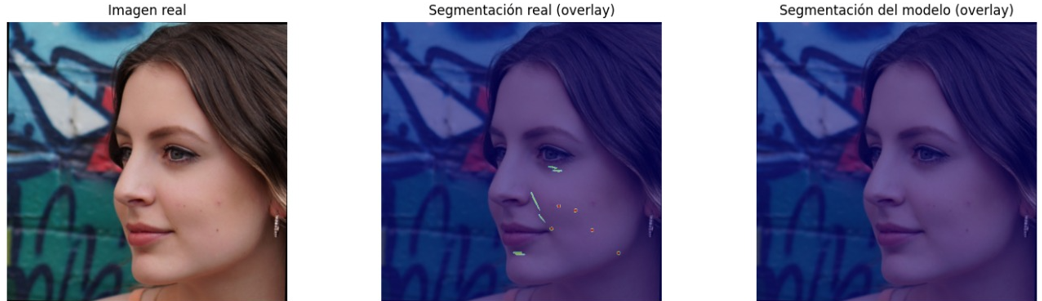
\includegraphics[width=0.75\textwidth]{4/figures/maskrcnn1.png}
      \caption{Comparación visual: imagen original, máscara real multicategoría y predicción del modelo 1.}
      \label{fig:validacionmaskrcnn1}
    \end{figure}
  
    \begin{figure}[H]
      \centering
      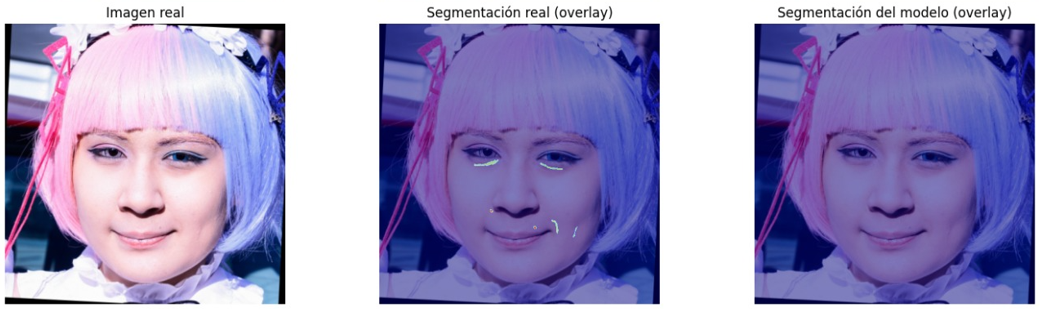
\includegraphics[width=0.75\textwidth]{4/figures/maskrcnn2.png}
      \caption{Comparación visual: imagen original, máscara real multicategoría y predicción del modelo 2.}
      \label{fig:validacionmaskrcnn2}
    \end{figure}
  
  
  \end{itemize}
  
  \vspace{0.2cm}
  En general, Mask R-CNN demostró ser una alternativa viable cuando se necesita detección de instancias separadas, aunque con un leve sacrificio en continuidad de segmentación para regiones difusas.
  


\end{enumerate}

Para poder comparar los resultados y métricas de los modelos de segmentación que se utilizaron se creo la siguiente Tabla \ref{tab:result_models}:
\begin{table}[H]
  \centering
  \caption{Comparación de Resultados y Métricas de rendimiento de los diferentes Modelos de Segmentación}
  \renewcommand{\arraystretch}{1.3}
  \begin{tabularx}{\textwidth}{@{}p{5cm} >{\centering\arraybackslash}X >{\centering\arraybackslash}X >{\centering\arraybackslash}X >{\centering\arraybackslash}X@{}}
      \toprule
      \textbf{Modelos} & \textbf{Entropía Cruzada (Loss)} & \textbf{Precisión} & \textbf{Índice de Sørensen–Dice} & \textbf{Coeficiente de Jaccard} \\ \midrule
      U-Net & 0.1849 & 0.832 & 0.712 & 0.759 \\
      U-Net Attention & 0.1158 & 0.911 & 0.810 & 0.852 \\
      U-Net con codificador MiT-B0 & 0.1441 & 0.443 & 0.320 & 0.470 \\
      Mask R-CNN & 0.4410 & 0.153 & 0.052 & 0.221 \\
      \bottomrule
  \end{tabularx}
  \label{tab:result_models}
\end{table}


Como se observa en la Tabla \ref{tab:result_models}, el modelo U-Net Attention presenta el mejor rendimiento global en la tarea de segmentación de arrugas y manchas faciales, al registrar la mayor precisión (0.911), así como los índices más altos de Sørensen–Dice (0.810) y Jaccard (0.852), junto con la menor pérdida por entropía cruzada (0.1158). Estos resultados reflejan una segmentación más precisa y coherente en comparación con los demás modelos evaluados. En contraste, Mask R-CNN mostró un desempeño significativamente inferior en todas las métricas, lo cual sugiere una menor capacidad para capturar adecuadamente los patrones de las características faciales sutiles. El modelo U-Net con codificador MiT-B0, si bien tiene una pérdida aceptable (0.1441), no logra alcanzar niveles óptimos de precisión ni superposición, lo que indica que el codificador MiT-B0, en este caso, no mejora el rendimiento como se esperaba. En general, los resultados evidencian que el uso de mecanismos de atención en arquitecturas U-Net potencia la capacidad de los modelos para segmentar estructuras faciales finas como arrugas y manchas, lo cual será crucial para la elección del mejor modelo en el despliegue.

\section{Despliegue del modelo}
\textbf{Actividad 1 de “\textit{Despliegue del modelo}”: Preparación del Entorno de Despliegue}
\\
El entorno de despliegue del sistema fue diseñado para ejecutarse localmente bajo una arquitectura cliente-servidor. Esta elección permite separar la lógica de interacción del usuario (frontend) de la lógica de procesamiento y predicción (backend), facilitando la escalabilidad y mantenibilidad del proyecto.
\\
\textbf{Configuración del entorno de desarrollo local:}
\\
Se definieron dependencias específicas del entorno Python para garantizar la ejecución adecuada del backend. Estas incluyen:
\begin{itemize}
\item \textbf{Flask:} para la construcción de una API RESTful ligera.
\item \textbf{PyTorch y torchvision:} para la inferencia del modelo y su manipulación.
\item \textbf{Opencv-python, numpy y Pillow:} para operaciones de procesamiento de imágenes.
\item \textbf{Albumentations:} para mantener el preprocesamiento coherente con el entrenamiento.
\item \textbf{Mediapipe:} (aunque se ejecuta en el cliente) puede formar parte del entorno general.
\end{itemize}
Se recomienda el uso de un entorno virtual para aislar las dependencias.

\textbf{Detección y configuración del dispositivo de cómputo:}

El sistema detecta automáticamente si hay disponibilidad de GPU (CUDA) usando \texttt{torch.cuda.is\_available()}. Si hay GPU, el modelo se carga y ejecuta sobre ella; de lo contrario, opera en CPU. Esto garantiza compatibilidad con diversos entornos, aunque con diferentes niveles de rendimiento.

\vspace{0.5em}
\textbf{Estructura de archivos y directorios del proyecto:}

\begin{itemize}
    \item \texttt{app.py}: archivo principal que lanza el servidor Flask, carga el modelo y procesa las peticiones.
    \item \texttt{templates/index.html}: plantilla HTML de la interfaz.
    \item \texttt{static/}: contiene archivos como \texttt{styles.css}, scripts JS y recursos visuales.
    \item \texttt{images/}: almacena imágenes temporales para depuración.
    \item \texttt{best\_model\_Unet\_attention\_Modificado\_150.pth}: pesos del modelo entrenado por 150 épocas.
\end{itemize}

\vspace{1em}
\textbf{Actividad 2 de “\textit{Despliegue del modelo}”: Despliegue del Modelo en Producción}

El sistema completo fue desplegado como una aplicación web local, permitiendo a los usuarios interactuar con el modelo mediante una interfaz gráfica accesible desde un navegador.

\textbf{Frontend – Captura e Interacción con el Usuario:}
\\
El frontend fue desarrollado con:
\begin{itemize}
\item HTML5 para estructura semántica.
\item CSS3 y Bootstrap para diseño responsivo.
\item JavaScript y JQuery para lógica e interactividad.
\item MediaPipe Face Detection para guiar al usuario a posicionar correctamente su rostro antes de capturar la imagen.
\end{itemize}

La lógica de detección facial se ejecuta en el cliente y valida en tiempo real si el rostro está correctamente centrado. Sólo cuando se detecta el rostro alineado, se habilita el botón de captura. Esta imagen se convierte en Base64 y se envía al backend vía POST a \texttt{/segment}.

\textbf{Backend – Inferencia del Modelo de Segmentación:}
\\
El backend, implementado con Flask, responde a las solicitudes del frontend. Al recibir una imagen codificada en Base64:
\begin{itemize}
\item La decodifica a formato PIL.Image.
\item Aplica transformaciones con Albumentations:
  \begin{itemize}
    \item Redimensionamiento a 256×256.
    \item Normalización con estadísticas de ImageNet.
    \item Conversión a tensor y agregación de dimensión de lote.
  \end{itemize}
\item Realiza la inferencia con el modelo UNet con Atención (UNetAttention), que utiliza:
    \begin{itemize}
    \item Bloques DoubleConv para extraer características.
    \item Attention Gates para enfocar regiones relevantes.
    \item ConvTranspose2d para reconstruir la imagen segmentada.
    \item Convolución final 1×1 para obtener 3 canales (fondo, arrugas, manchas).
  \end{itemize}
\item Aplica \texttt{torch.argmax} sobre la salida para obtener la clase más probable por píxel.
\item Genera una máscara coloreada: manchas en rojo, arrugas en azul.
\item Superpone la máscara sobre la imagen original y la convierte nuevamente a Base64.
\end{itemize}

\textbf{Visualización de Resultados:}
El frontend recibe la imagen segmentada con overlay y la muestra dinámicamente los siguientes frames: 
\begin{itemize}
  \item El usuario puede ver el primer frame visual como presentación de la página como se ve en la Figura \ref{fig:presinicial}.

\begin{figure}[H]
      \centering
      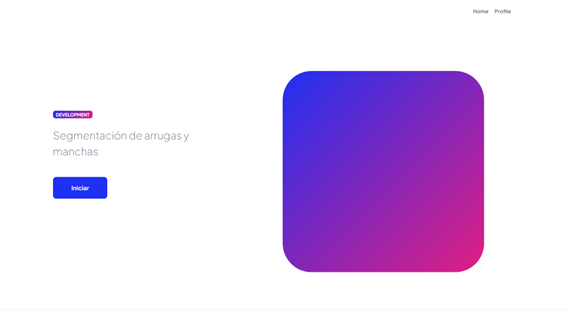
\includegraphics[width=1\textwidth]{4/figures/PresentacionInicialPage.png}
      \caption{Presentación inicial de la página.}
      \label{fig:presinicial}
    \end{figure}

\item El usuario puede ver la notificación de que todo está bien al tomar la foto de su rostro en la posición correcta como se ve en la Figura \ref{fig:prescamact}.
\begin{figure}[H]
      \centering
      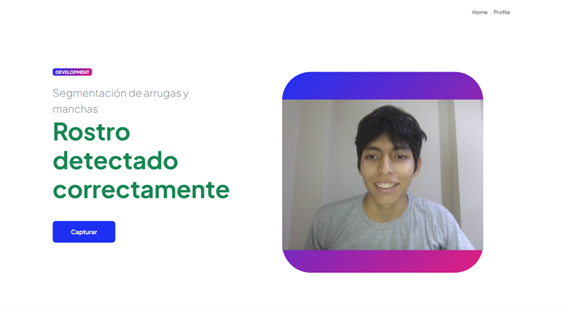
\includegraphics[width=1\textwidth]{4/figures/PresCamActive.png}
      \caption{Presentación con cámara activa.}
      \label{fig:prescamact}
    \end{figure}

\item El usuario puede ver en tiempo real las regiones detectadas gracias al sistema de retroalimentación visual como se ve en la Figura \ref{fig:presseg}.

\begin{figure}[H]
      \centering
      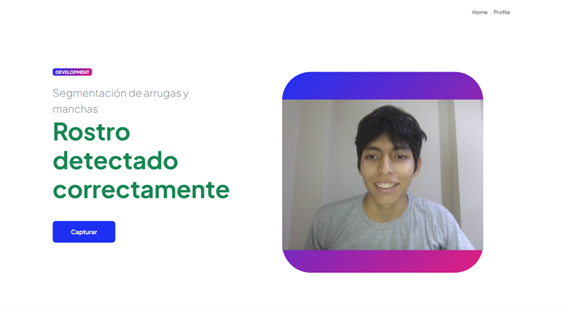
\includegraphics[width=1\textwidth]{4/figures/PresCamActive.png}
      \caption{Presentación de la segmentación.}
      \label{fig:presseg}
    \end{figure}

  \end{itemize}
\textbf{Errores y control de flujo:}
Si ocurre algunos de los siguientes errores en la captura de imagen para la futura segmentación, el sistema notifica al usuario con una alerta:

\begin{itemize}
  \item La no aparición o presentación de un rostro facil en la cámara web como se ve en la Figura \ref{fig:sincam}.
\begin{figure}[H]
      \centering
      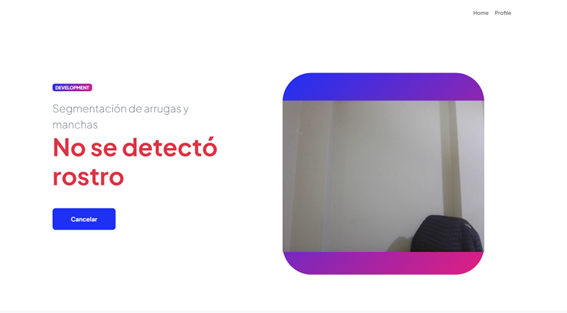
\includegraphics[width=1\textwidth]{4/figures/PresSinCam.png}
      \caption{Presentación cuando no hay un rostro.}
      \label{fig:sincam}
    \end{figure}
  \item El no tener centrado el rostro en la cámara web para una recomendada segmentación de las deformaciones morfológicas faciales como se ve en la Figura \ref{fig:presfueracam}.

\begin{figure}[H]
      \centering
      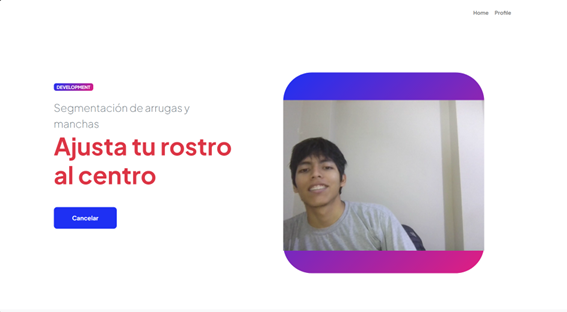
\includegraphics[width=1\textwidth]{4/figures/PresCamFuer.png}
      \caption{Presentación cuando el rostro no está en el centro.}
      \label{fig:presfueracam}
    \end{figure}
  \end{itemize}



